\chapter{THIẾT KẾ}
\section{Mô Hình Công Nghệ}
\subsection{Tổng quan công nghệ}
\subsubsection{WebSocket}
WebSocket là một giao thức được phổ biến cho việc phát triển ứng dụng real-time, cho phép các trình duyệt giao tiếp với nhau theo thời gian thực. Giao thức WebSocket  cung cấp một cách thức để tạo những kết nối bền bỉ, độ trễ thấp để hỗ trợ giao tiếp giữa client và server (giap tiếp hai chiều - two way communication). Sử dụng WebSockets có thể tạo một ứng dụng \textbf{real-time} đúng nghĩa như ứng dụng chat, sử dụng 1 tiến trình để nói chuyện với tiến trình khác, phối hợp soạn thảo văn bản, giao dịch chứng khoán hay game online nhiều người chơi cùng lúc.
\par Một chức năng khác của socket là giúp các tầng \textbf{TCP} định danh ứng dụng mà dữ liệu sẽ được gửi tới thông qua sự ràng buộc với một cổng port (thể hiện là một con số cụ thể), từ đó tiến hành kết nối giữa client và server.

	\begin{center}
	\begin{figure}[H]
		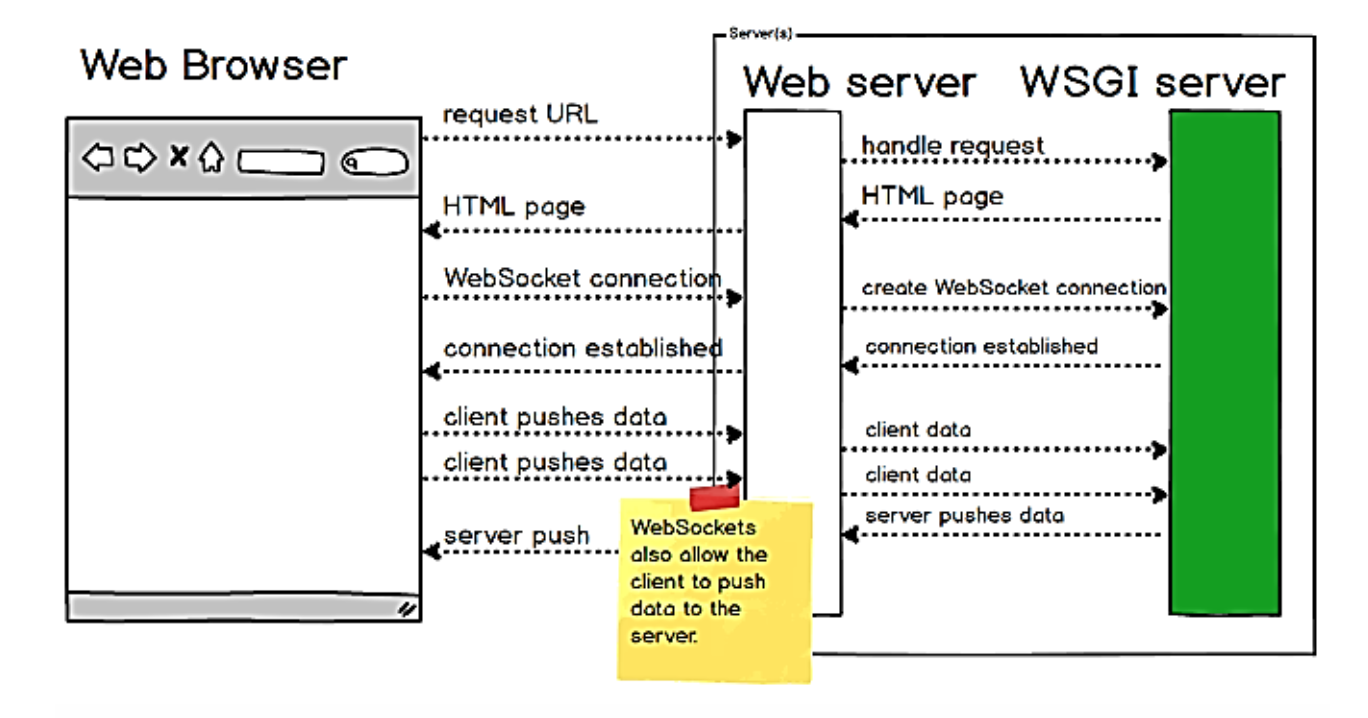
\includegraphics[width=17cm]{{./imgs/WebSocket_structure}}
		\caption{Sơ đồ hoạt động của WebSocket}
	\end{figure}
	\end{center}  
\subsubsection{Giao thức TCP/IP}
	\begin{center}
	\begin{figure}[H]
		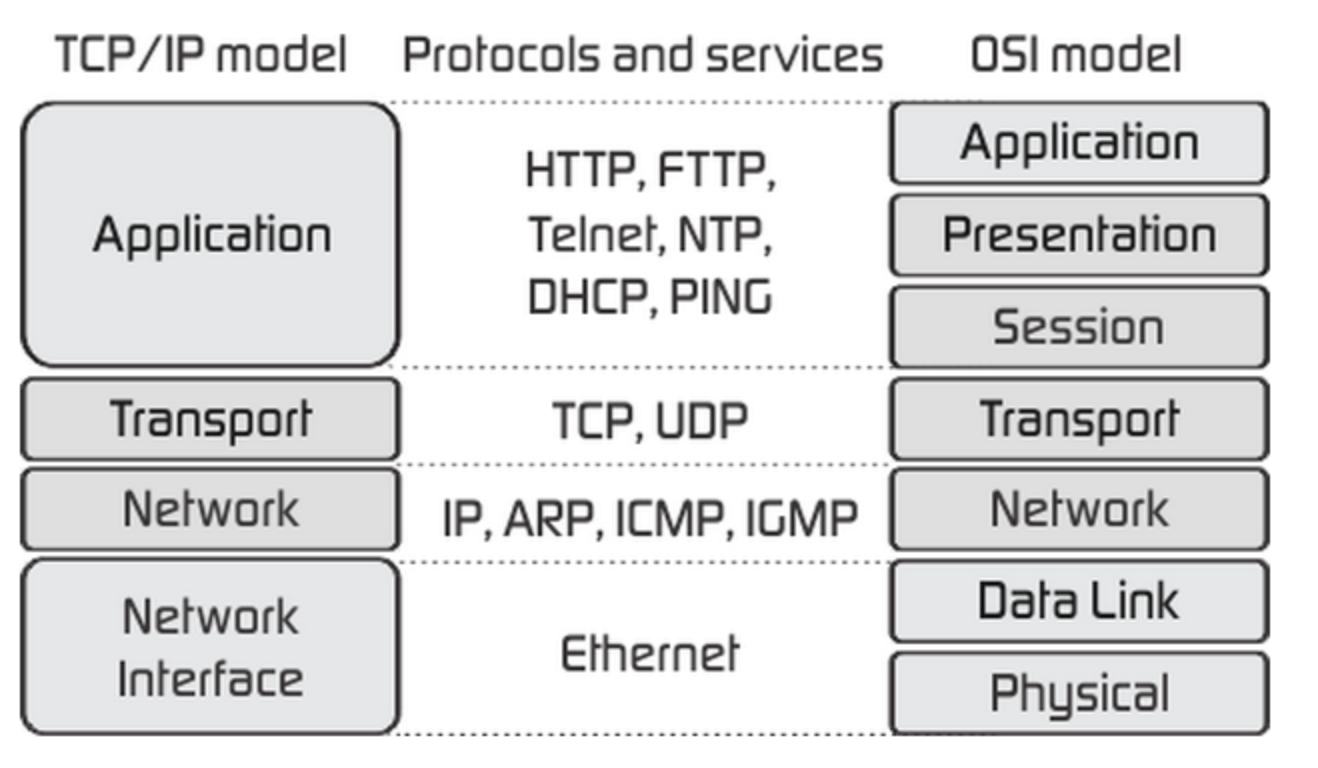
\includegraphics[width=17cm]{{./imgs/TCP_OSI}}
		\caption{TCP/IP với mô hình OSI}
	\end{figure}
	\end{center} 


\paragraph{Giao thức được chia thành các tầng mạng trong mô hình OSI}
	\begin{itemize}
       \item \textbf{Tầng Application}: Nhiệm vụ của tầng này đó là cung cấp các ứng dụng, trao đổi dữ liệu được chuẩn hóa. Trong tầng ứng dụng bao gồm nhiều giao thức cụ thể như HTTP, FTP, POP3, SMTP, SNMP. Mỗi giao thức này sẽ có chức năng và nhiệm vụ cụ thể.
        \item \textbf{Tầng Network}: Nhiệm vụ của tầng internet là xử lý các gói tin, sau đó kết nối với các mạng độc lập để vận chuyển các gói dữ liệu đã được mã hóa qua các ranh giới mạng.
        \item \textbf{Tầng Transport}: Nhiệm vụ của tầng giao vận là duy trì liên lạc đầu cuối trên toàn mạng. Tầng giao vận bao gồm giao thức \textbf{TCP và UDP}. Trong nhiều trường hợp giao thức UDP sẽ được thay thế TCP.
       \end{itemize}
      
     \begin{center}
	\begin{figure}[H]
		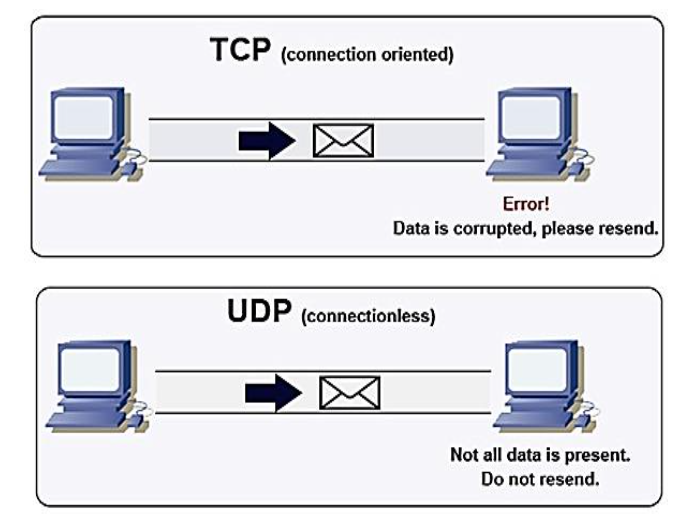
\includegraphics[width=17cm]{{./imgs/TCP_UDP_flow}}
		\caption{Cách thức truyền nhận dữ liệu}
	\end{figure}
	\end{center}  
  \par Nguyên lý hoạt động của giao thức này là sự kết hợp giữa hai giao thức riêng biệt, đó là giữa giao thức kiểm soát truyền tin và giao thức internet. Đầu tiên giao thức IP sẽ cho phép các gói tin được gửi qua mạng bằng cách cho biết những gói tin này được gửi qua đâu và làm như thế nào. \par
 Ngay sau khi được yêu cầu giao thức IP sẽ điều khiển truyền dẫn để giúp truyền những dữ liệu đáng tin cậy thông qua các kết nối mạng internet. Cuối cùng giao thức TCP sẽ kiểm tra lại các gói dữ liệu một lần nữa xem có lỗi và xảy ra vấn đề gì không. Nếu không có lỗi thì sẽ truyền đến vị trí cần thiết, trong trường hợp có lỗi thì sẽ gửi lại yêu cầu truyền lại.

\subsubsection{NodeJS}
NodeJS là một nền tảng được xây dựng trên \textbf{V8 JavaScript Engine} – trình thông dịch thực thi mã JavaScript, giúp xây dựng các ứng dụng web một cách đơn giản và dễ dàng mở rộng. \par
NodeJS được phát triển bởi Ryan Dahl vào năm 2009 và có thể chạy trên nhiều hệ điều hành khác nhau: OS X, Microsoft Windows, Linux. Các ưu điểm của NodeJS.
\begin{itemize}
       \item NodeJS được viết bằng JavaScript với cộng đồng người dùng lớn mạnh.
        \item Tốc độ xử lý nhanh. Nhờ cơ chế xử lý \textbf{bất đồng độ (non-blocking)}, NodeJS có thể xử lý hàng ngàn kết nối cùng lúc mà không gặp bất cứ khó khăn nào.
        \item Dễ dàng mở rộng.
       \end{itemize}

\subsubsection{MySQL}
MySQL là chương trình dùng để quản lý hệ thống cơ sở dữ liệu (CSDL), trong đó CSDL là một hệ thống lưu trữ thông tin. được sắp xếp rõ ràng, phân lớp ngăn nắp những thông tin mà mình lưu trữ. Các ưu điểm của MySQL.
\begin{itemize}
       \item Khả năng mở rộng và tính linh hoạt.
        \item Hiệu năng cao.
        \item Bảo vệ dữ liệu mạnh mẽ.
        \item Tính sẵn sàng cao.
        \item Mã nguồn mở tự do
       \end{itemize}

%%%%%%%%%%%%%%%%%%%%%%%%%%%%%%%%
\section{Mô Hình Triển Khai}

	\begin{center}
	\begin{figure}[H]
		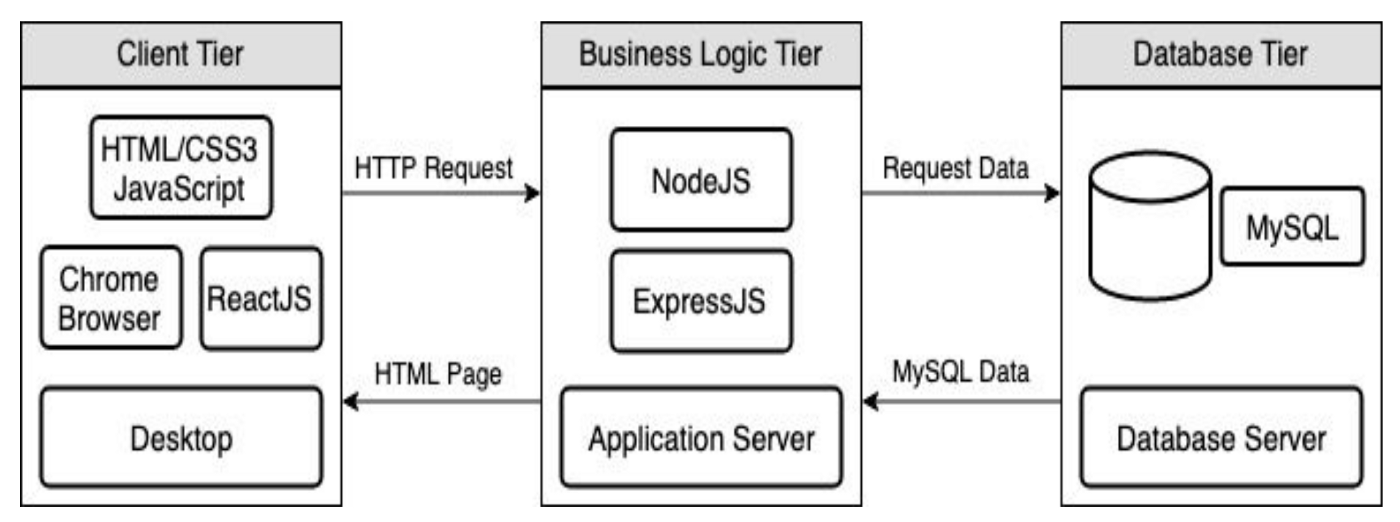
\includegraphics[width=17cm]{{./imgs/implement_diagram}}
		\caption{Mô hình triển khai công nghệ}
	\end{figure}
	\end{center}
	
	\begin{center}
	\begin{figure}[H]
		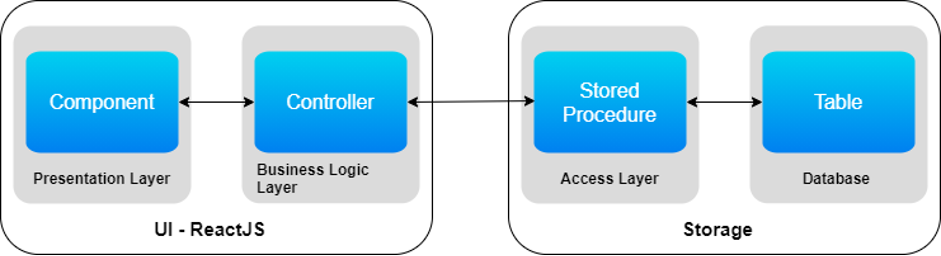
\includegraphics[width=17cm]{{./imgs/technoligy_diagram}}
		\caption{Sơ đồ luồng dữ liệu}
	\end{figure}
	\end{center}

\begin{center}
\begin{longtabu} to \textwidth {| m{5cm} | m{5cm} | m{5cm} |}
\caption{Mô tả sơ đồ} \\
\hline \textbf{Tên đối tượng} & \textbf{Mô tả} & \textbf{Yêu cầu} \\ \hline
\endfirsthead
\hline \textbf{Tên đối tượng} & \textbf{Mô tả} & \textbf{Yêu cầu} \\ \hline
\endhead
\hline
\endfoot
Client Tier & Phía giao diện sẽ được viết bằng HTML, CSS, Javascript \& thư viện ReactJS & Tương tác \& truy cập tới các tính năng của ứng dụng 
\\ \hline
Business Logic Tier & Phía Server sẽ được phát triển bằng NodeJS \& ExpressJS như 1 cầu nối giao tiếp tới giao diện và cơ sở dữ liệu & Tiếp nhận các yêu cầu HTTP được gửi từ người dùng và gửi phản hồi thích hợp
\\ \hline
Database Tier & Dùng cơ sở dữ liệu MySQL để lưu trữ & Lưu trữ tất cả dữ liệu của ứng dụng
\end{longtabu}
\end{center}
	
%%%%%%%%%%%%%%%%%%%%%%%%%5

\section{Thiết Kế Giao Diện}
\subsection{Sitemap}
	\begin{center}
		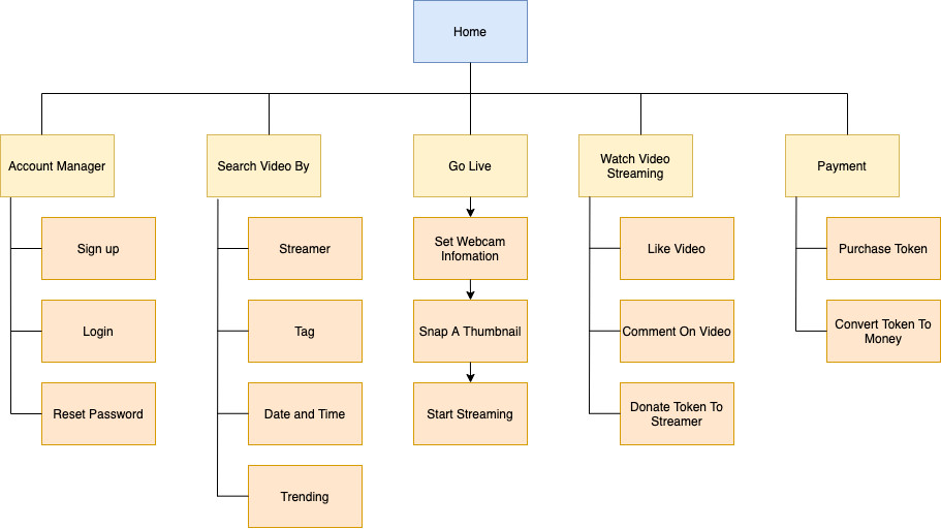
\includegraphics[scale=1]{{./imgs/sitemap.png}}
	\end{center}

\begin{center}
\begin{longtabu} to \textwidth {| m{4cm} | m{5cm} | m{6cm} |}
\caption{Mô tả sitemap}  \\ 
\hline
\multicolumn{1}{|c|}{\textbf{Tên}}              & \multicolumn{1}{c|}{\textbf{Chức năng}} & \multicolumn{1}{c|}{\textbf{Mô tả}} \\ \hline
\multirow{3}{*}{Account manager}       & Sign up                        & Đăng ký tài khoản          \\ \cline{2-3} 
                                       & Login                          & Đăng nhập vào hệ thống     \\ \cline{2-3} 
                                       & Reset password                 & Đổi mật khẩu               \\ \hline
\multirow{4}{*}{Search video}          & Streamer                       & Tìm kiếm theo streamer     \\ \cline{2-3} 
                                       & Tag                            & Tìm kiếm theo tag          \\ \cline{2-3} 
                                       & Date and time                  & Tìm kiếm theo thời gian    \\ \cline{2-3} 
                                       & Trending                       & Tìm kiếm theo thịnh hành   \\ \hline
\multirow{3}{*}{Go live}               & Set webcam information         & Thiết lập thông tin video  \\ \cline{2-3} 
                                       & Snap a thumbnail               & Chụp thumbnail cho video   \\ \cline{2-3} 
                                       & Start streaming                & Bắt đầu stream             \\ \hline
\multirow{3}{*}{Watch video streaming} & Like video                     & Thích video                \\ \cline{2-3} 
                                       & Comment on video               & Viết bình luận cho video   \\ \cline{2-3} 
                                       & Donate token to streamer       & Tặng token cho streamer    \\ \hline
\multirow{2}{*}{Payment}               & Purchase token                 & Mua token                  \\ \cline{2-3} 
                                       & Convert                        & Quy đổi token              \\ \hline
\end{longtabu}
\end{center}
	
\subsection{Giao diện chức năng}
	\begin{center}
	\begin{figure}[H]
		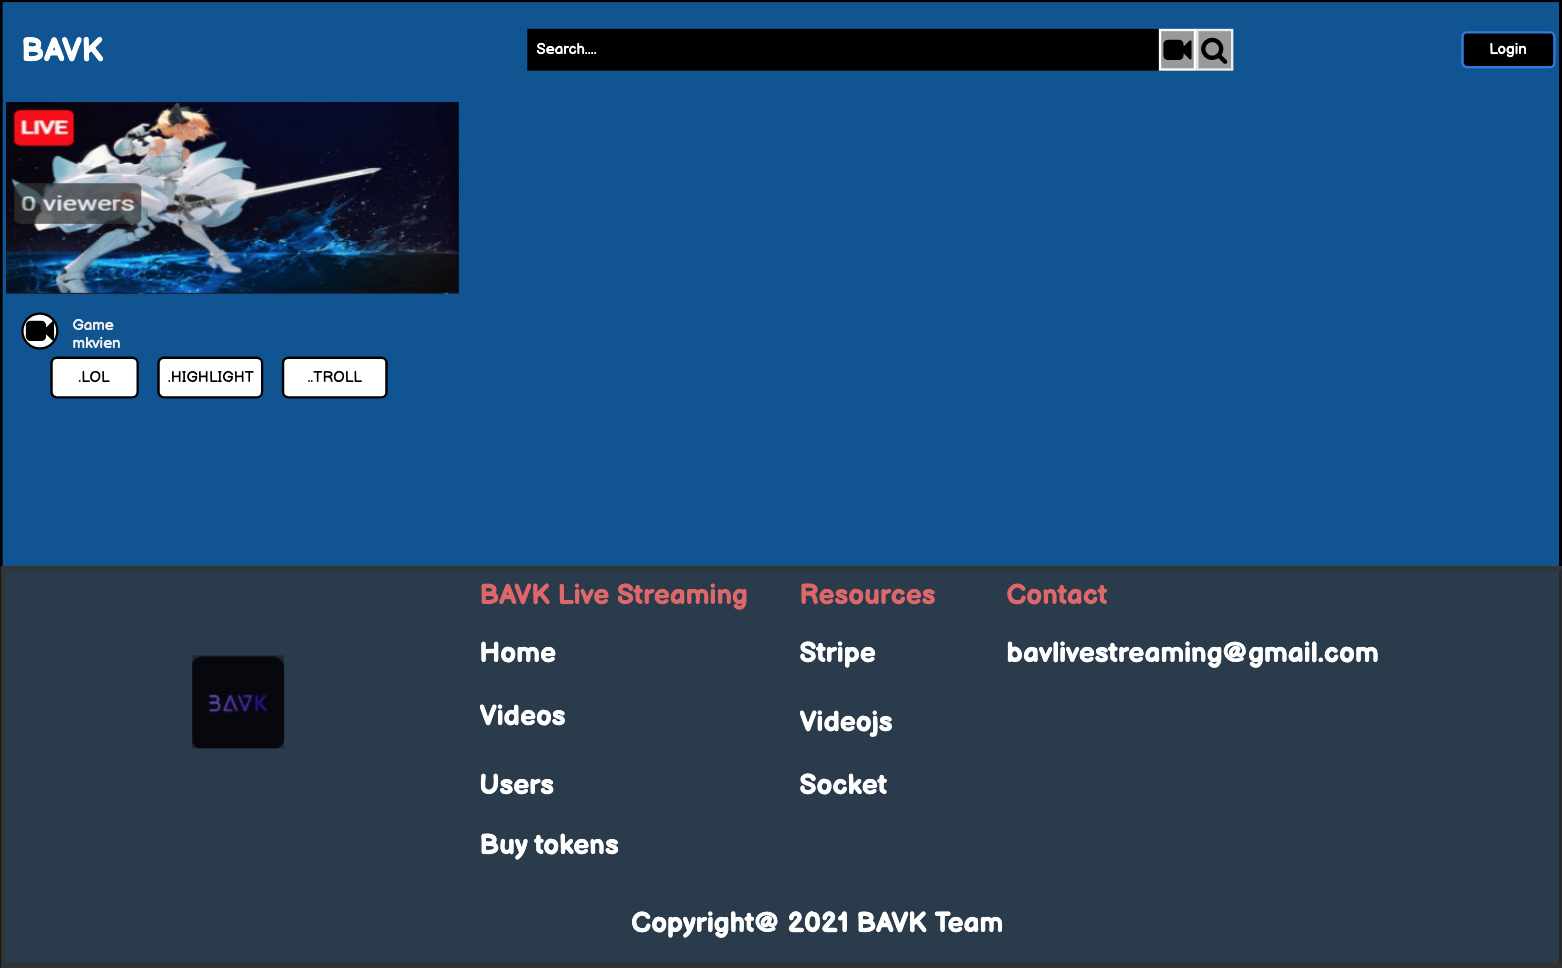
\includegraphics[width=17cm]{{./imgs/landing_page}}
		\caption{Trang chủ}
	\end{figure}
	\end{center}
	
\begin{center}
\begin{longtabu} to \textwidth {| m{1cm} | m{4cm} | m{3cm} | m{7cm} |}
\caption{Mô tả trang chủ} \\
    \hline \textbf{STT}  & \textbf{Điều khiển} & \textbf{Sự kiện} & \textbf{Mô tả} \\ \hline
    \endfirsthead
    \hline \textbf{STT}  & \textbf{Điều khiển} & \textbf{Sự kiện} & \textbf{Mô tả} \\ \hline
    \endhead
      1 & Search bar  & Input & Tìm kiếm tương đối các thông tin liên quan từ khóa người dùng nhập vào \\
      \hline
      2 & Video list & Initialize & Hiển thị các video đang được streaming  \\
      \hline
      3 & Footer  & Initialize & Chứa các thông tin chung, bản quyền của website \\
      \hline
\end{longtabu}
\end{center}
	
	\begin{center}
	\begin{figure}[H]
		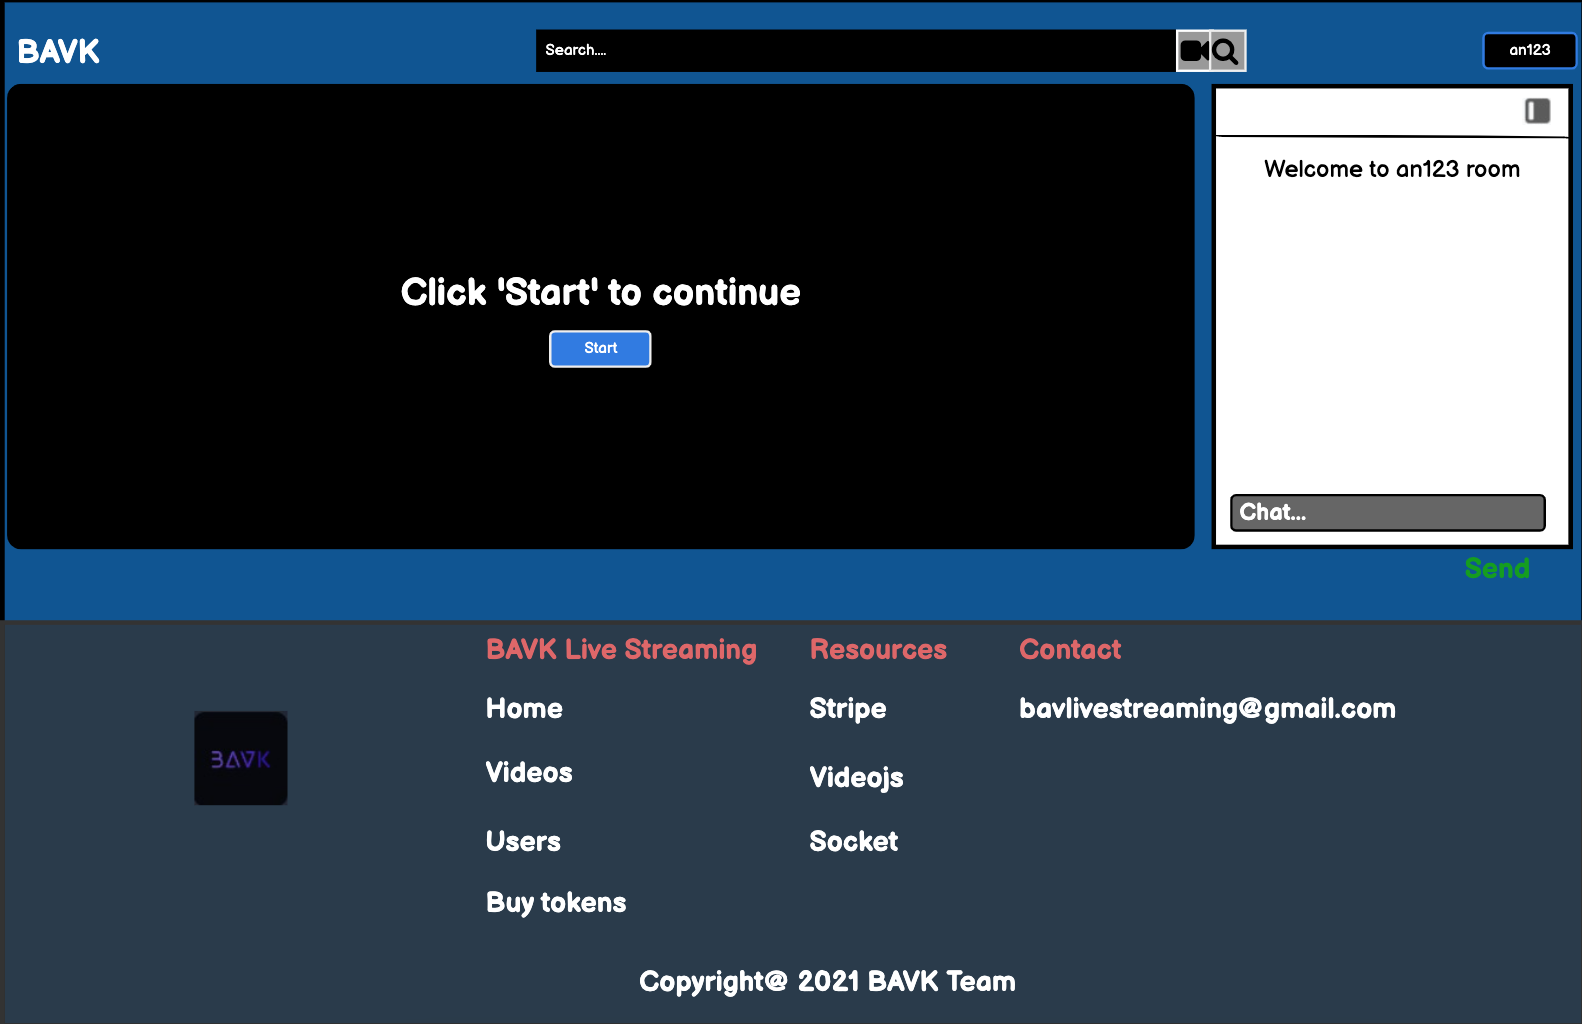
\includegraphics[width=17cm]{{./imgs/streamer_page}}
		\caption{Trang cho streamer}
	\end{figure}
	\end{center}
	
	
\begin{center}
\begin{longtabu} to \textwidth {| m{1cm} | m{4cm} | m{3cm} | m{7cm} |}
\caption{Mô tả trang streamer} \\
    \hline \textbf{STT}  & \textbf{Điều khiển} & \textbf{Sự kiện} & \textbf{Mô tả} \\ \hline
    \endfirsthead
    \hline \textbf{STT}  & \textbf{Điều khiển} & \textbf{Sự kiện} & \textbf{Mô tả} \\ \hline
    \endhead
      1 & Video manager  & Initialize & Hiển thị nội dung webcam thu được/ Hiển thị khu vực để stream trên màn hình \\
      \hline
      2 & Chat panel & Input/Click & Hiển thị các tin nhắn của tất cả người dùng trong kênh stream và cho phép người streamer tương tác với viewer \\
      \hline
      3 & Media player navigator & Click & Cho phép tin nhắn hiển thị trân màn hình stream, tắt/bật mic, cho phép truyền âm thanh, tắt/bật webcam 
      \\ \hline
       4 & Thông tin đang live stream & Initialize & Cho phép xem thông tin tiêu đề, số lượt xem, số lượng yêu thích, tổng thời gian đã live stream, các users đang bị lock chat
      \\ \hline
      5 & Ghi hình & Click & Cho phép streamer ghi hình lại video và sau đó có thể thiết lập các thông tin cần thiết để lưu video
      \\ \hline
\end{longtabu}
\end{center}
	

	\begin{center}
	\begin{figure}[H]
		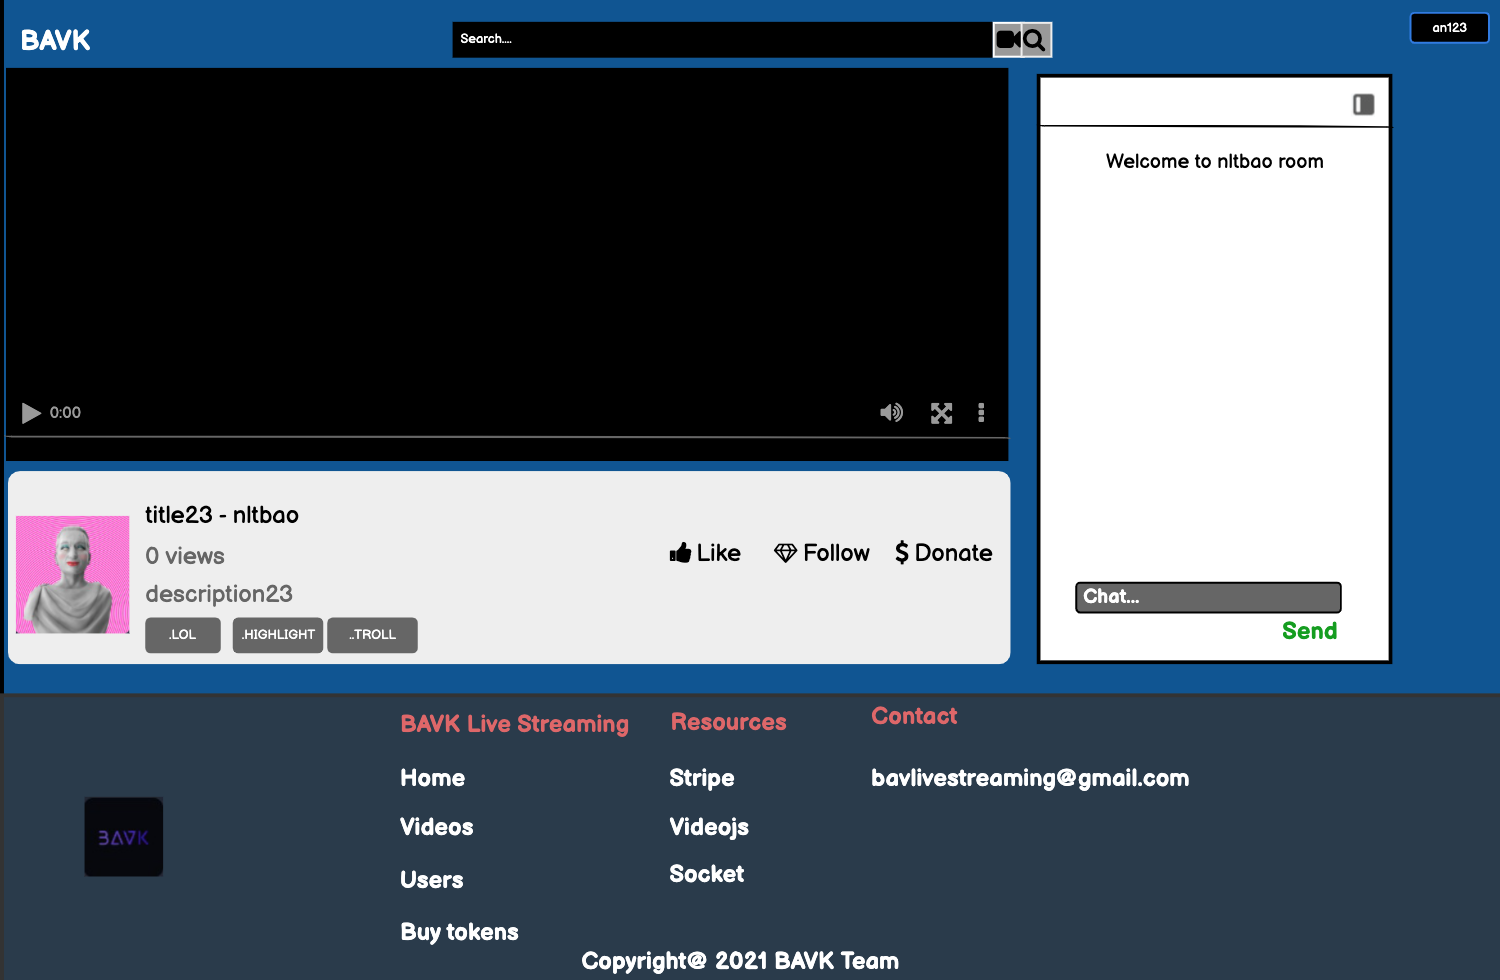
\includegraphics[width=17cm]{{./imgs/viewer_page}}
		\caption{Trang cho viewer}
	\end{figure}
	\end{center}

\begin{center}
\begin{longtabu} to \textwidth {| m{1cm} | m{4cm} | m{3cm} | m{7cm} |}
\caption{Mô tả trang viewer} \\
    \hline \textbf{STT}  & \textbf{Điều khiển} & \textbf{Sự kiện} & \textbf{Mô tả} \\ \hline
    \endfirsthead
    \hline \textbf{STT}  & \textbf{Điều khiển} & \textbf{Sự kiện} & \textbf{Mô tả} \\ \hline
    \endhead
      1 & Video player  & Initialize & Hiển thị hình ảnh đang được streamer chia sẻ \\
      \hline
      2 & Chat panel & Input/Click & Hiển thị các tin nhắn của tất cả người dùng trong kênh stream và cho phép người viewer tương tác với tất cả \\
      \hline
      3 & Streamer info & Click & Cho phép viewer theo dõi thông tin của streamer được chọn \\
      \hline
      4 & Subscribe button & Click & Đăng ký kênh, viewer sẽ nhận được các thông báo về các sự kiện liên quan của streamer khi có video \\
      \hline
      5 & Like video button & Click & Thích video đang xem  \\
      \hline
\end{longtabu}
\end{center}


	\begin{center}
	\begin{figure}[H]
		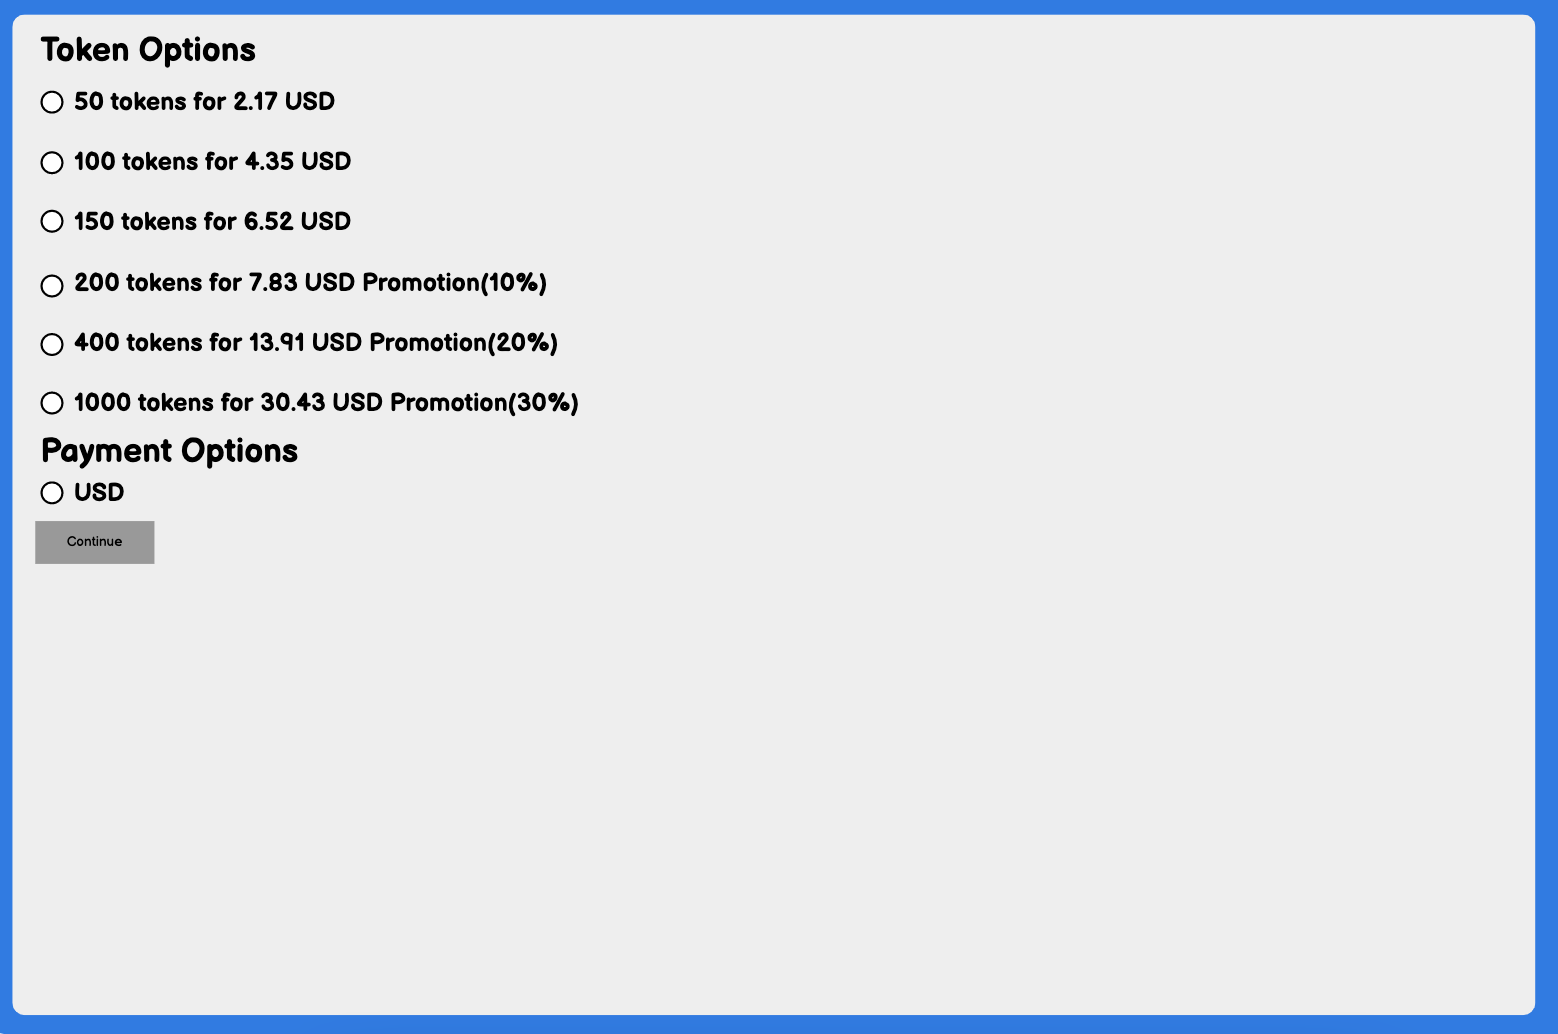
\includegraphics[width=17cm,height=15cm]{{./imgs/purchase_page}}
		\caption{Trang mua token}
	\end{figure}
	\end{center}
	
\begin{center}
\begin{longtabu} to \textwidth {| m{1cm} | m{4cm} | m{3cm} | m{7cm} |}
\caption{Mô tả trang mua token} \\
   \hline \textbf{STT}  & \textbf{Điều khiển} & \textbf{Sự kiện} & \textbf{Mô tả} \\ \hline
    \endfirsthead
    \hline \textbf{STT}  & \textbf{Điều khiển} & \textbf{Sự kiện} & \textbf{Mô tả} \\ \hline
    \endhead
      1 & Số lượng token muốn mua & Click & Người dùng có thể chọn số lượng token và đơn vị tiền tệ (USD) để thanh toán \\
      \hline
      2 & Tiến hành thanh toán & Input/Click & Người dùng thanh toán qua VISA \\
      \hline
\end{longtabu}
\end{center}


	\begin{center}
	\begin{figure}[H]
		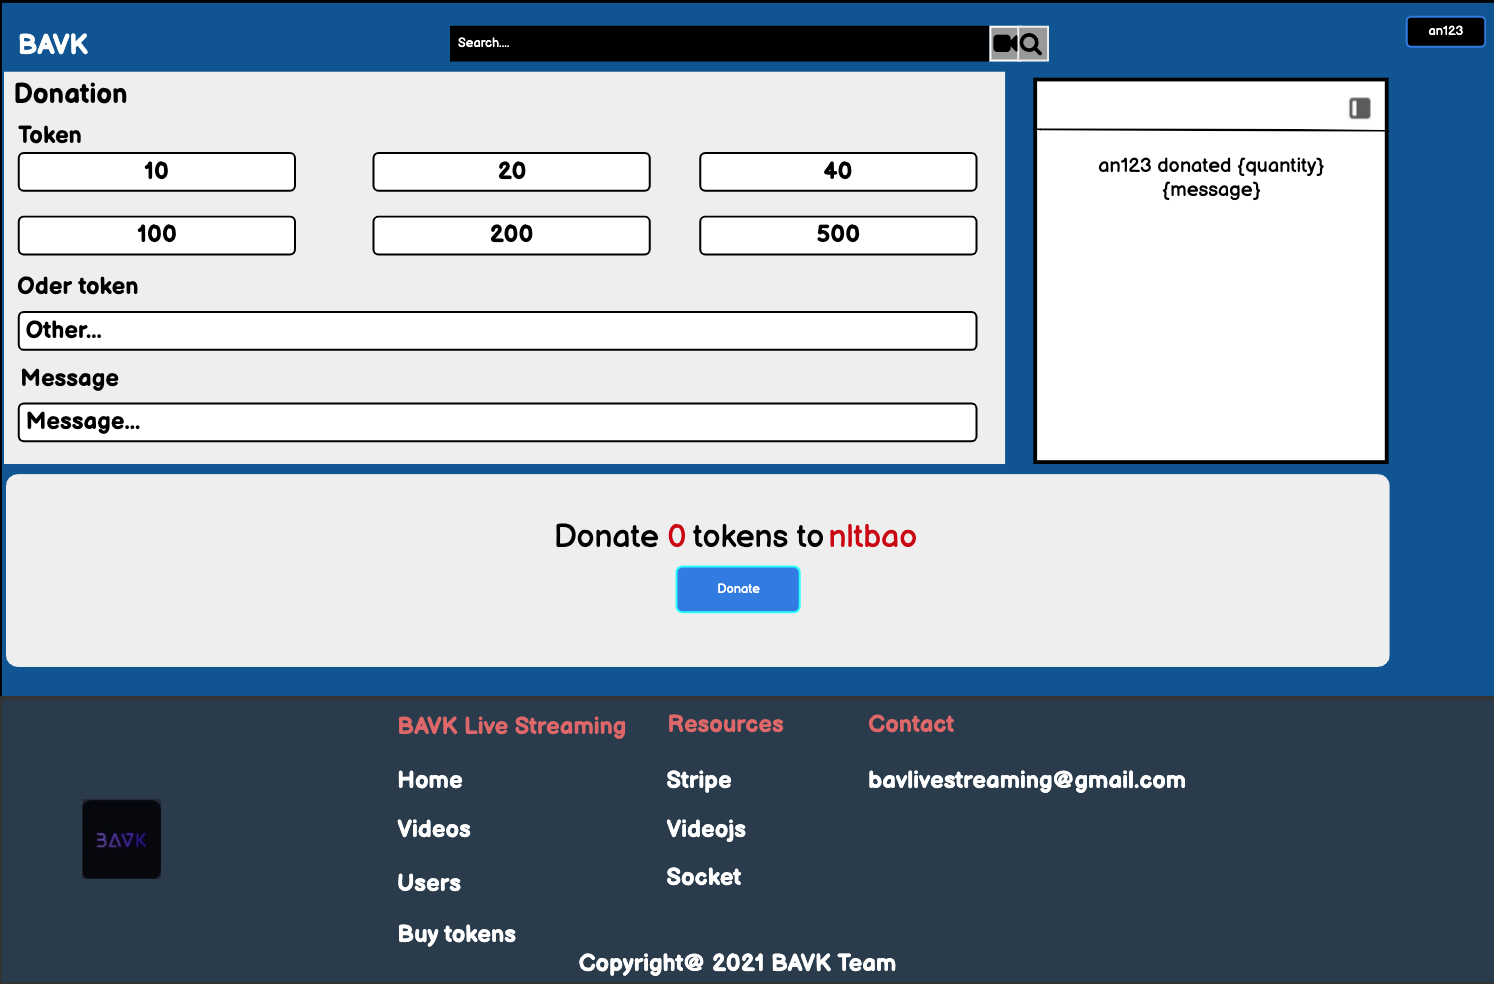
\includegraphics[width=17cm]{{./imgs/donate_page}}
		\caption{Trang donate}
	\end{figure}
	\end{center}
	
\begin{center}
\begin{longtabu} to \textwidth {| m{1cm} | m{4cm} | m{3cm} | m{7cm} |}
\caption{Mô tả trang donate} \\
    \hline \textbf{STT}  & \textbf{Điều khiển} & \textbf{Sự kiện} & \textbf{Mô tả} \\ \hline
    \endfirsthead
    \hline \textbf{STT}  & \textbf{Điều khiển} & \textbf{Sự kiện} & \textbf{Mô tả} \\ \hline
    \endhead
      1 & Số lượng token donate & Click & Cho phép nhân viên chọn số lượng token để đonate cho streamer(Số lượng donate phải phù hợp với số lượng token đang có) \\
      \hline
      2 & Tin nhắn gửi tới streamer & Input  & Cho phép người dùng gửi token đính kèm tin nhắn tới cho streamer \\
      \hline
      3 & Donate & Click & Sau khi donate, thông tin donate sẽ gửi trực tiếp broadcast tới phòng của streamer. Streamer và các viewer đều có thể thấy được tin nhắn \\
      \hline
\end{longtabu}
\end{center}	
	
	
	\begin{center}
	\begin{figure}[H]
		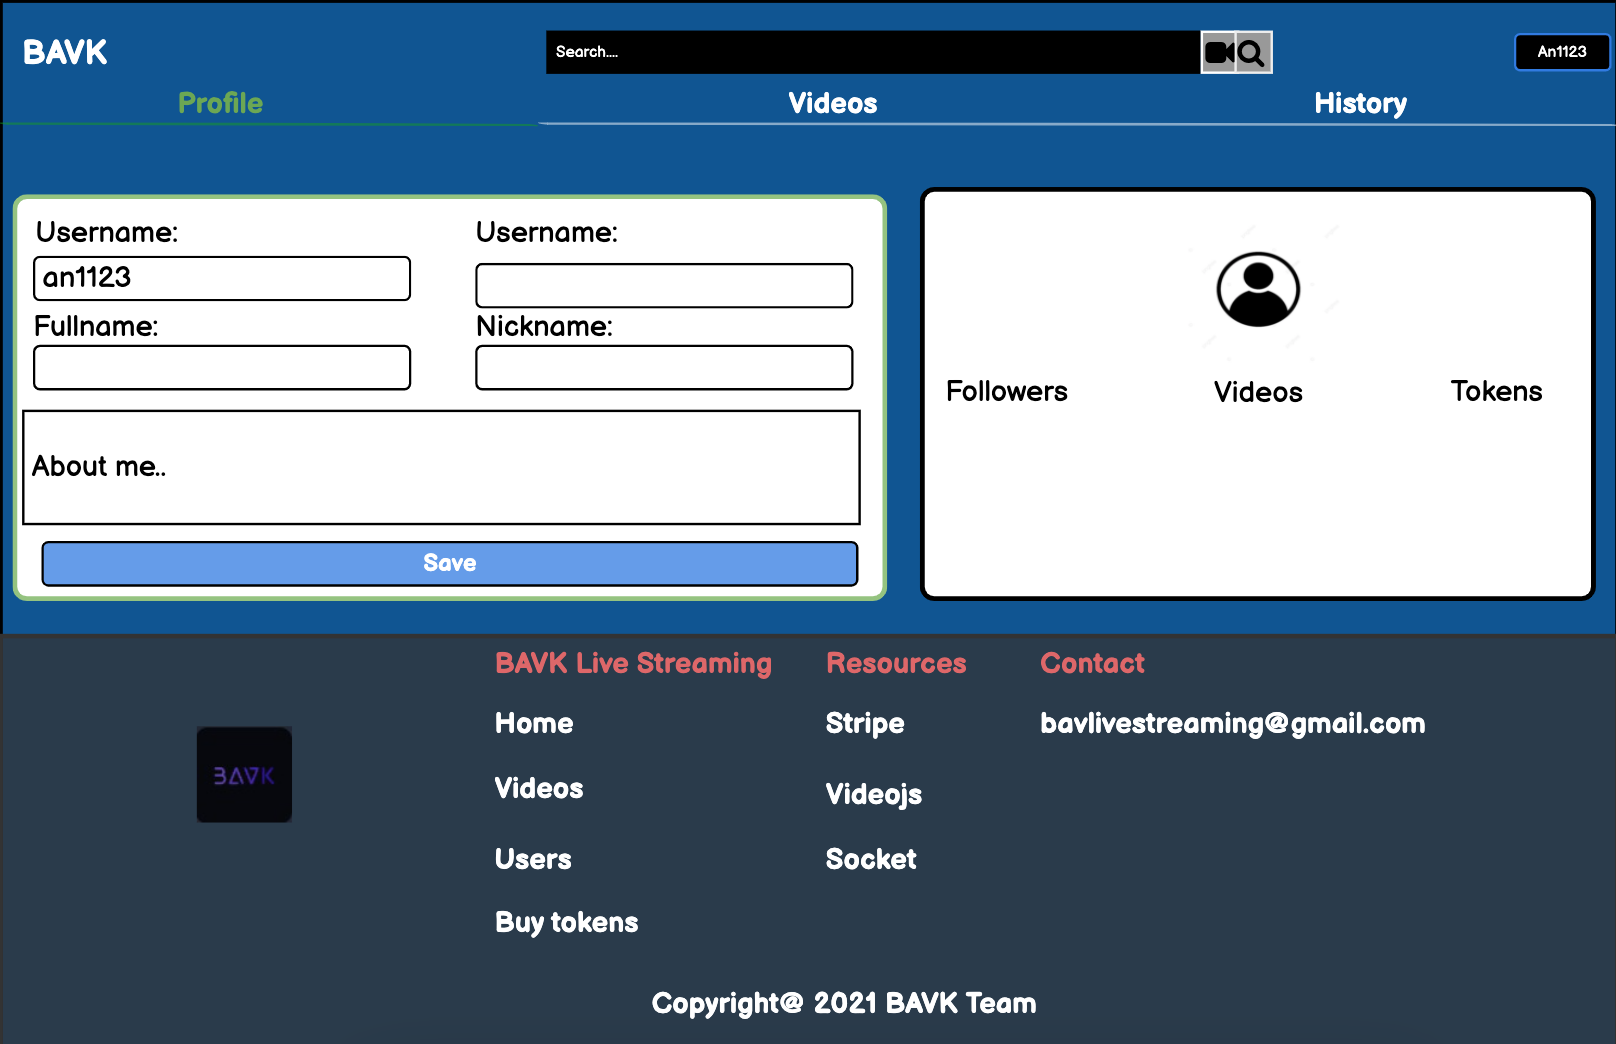
\includegraphics[width=17cm]{{./imgs/profile_page}}
		\caption{Trang hồ sơ}
	\end{figure}
	\end{center}
	
\begin{center}
\begin{longtabu} to \textwidth {| m{1cm} | m{4cm} | m{3cm} | m{7cm} |}
\caption{Mô tả trang thông tin cá nhân} \\
    \hline \textbf{STT}  & \textbf{Điều khiển} & \textbf{Sự kiện} & \textbf{Mô tả} \\ \hline
    \endfirsthead
    \hline \textbf{STT}  & \textbf{Điều khiển} & \textbf{Sự kiện} & \textbf{Mô tả} \\ \hline
    \endhead
      1 & Xem và thay đổi thông tin hồ sơ  & Initialize & Cho phép người dùng thay đổi thông tin \\
      \hline
      2 & Lưu hồ sơ& Click & Tiến hành thay đổi thông tin \\
      \hline
\end{longtabu}
\end{center}	


	\begin{center}
	\begin{figure}[H]
		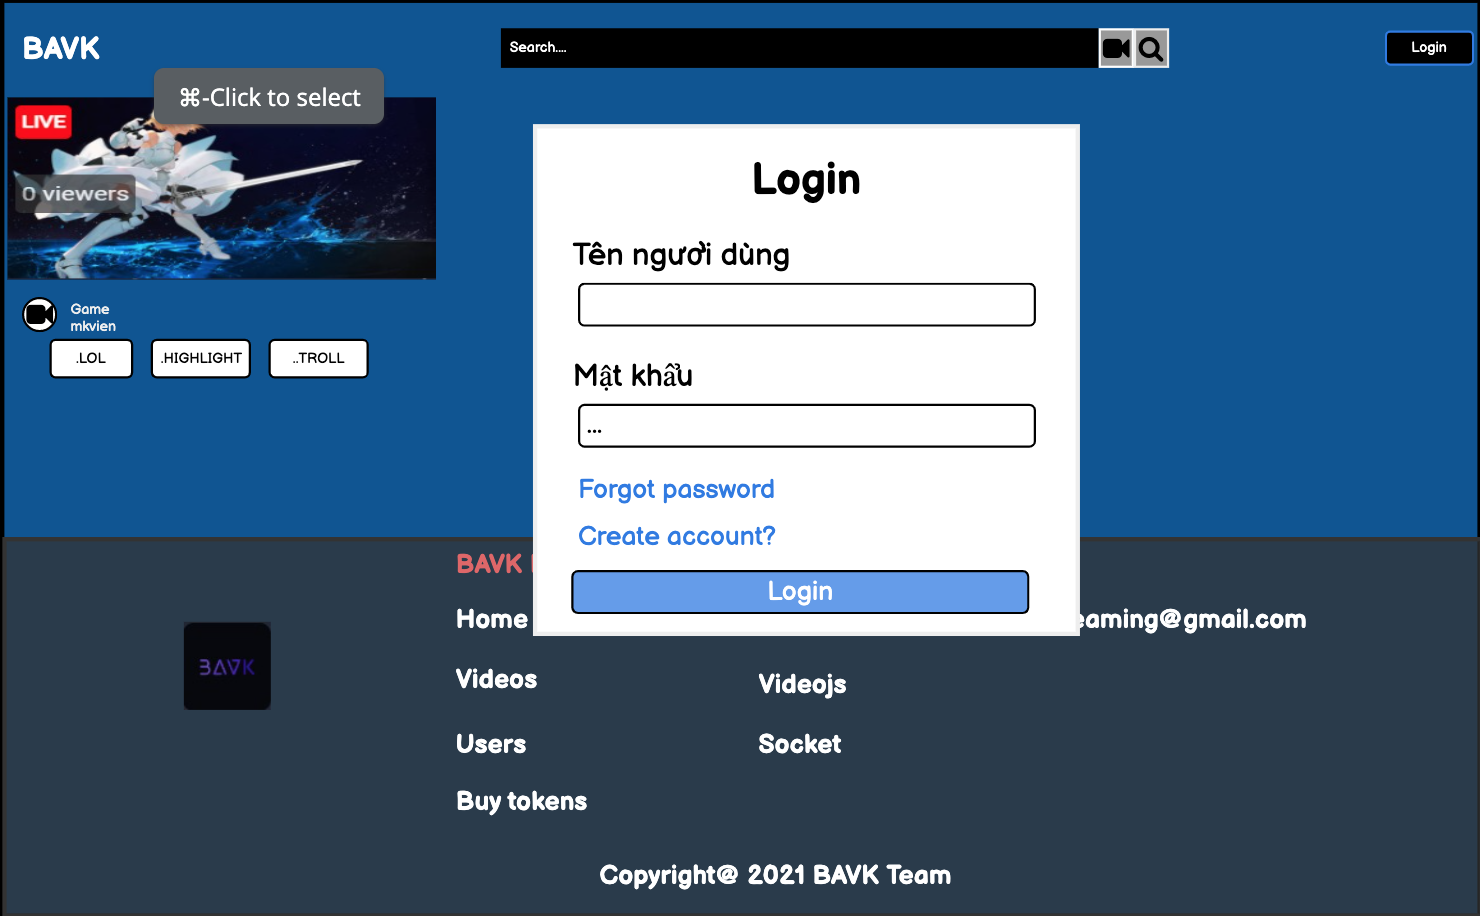
\includegraphics[width=17cm]{{./imgs/login_page}}
		\caption{Trang đăng nhập}
	\end{figure}
	\end{center}
	\begin{center}
	\begin{figure}[H]
		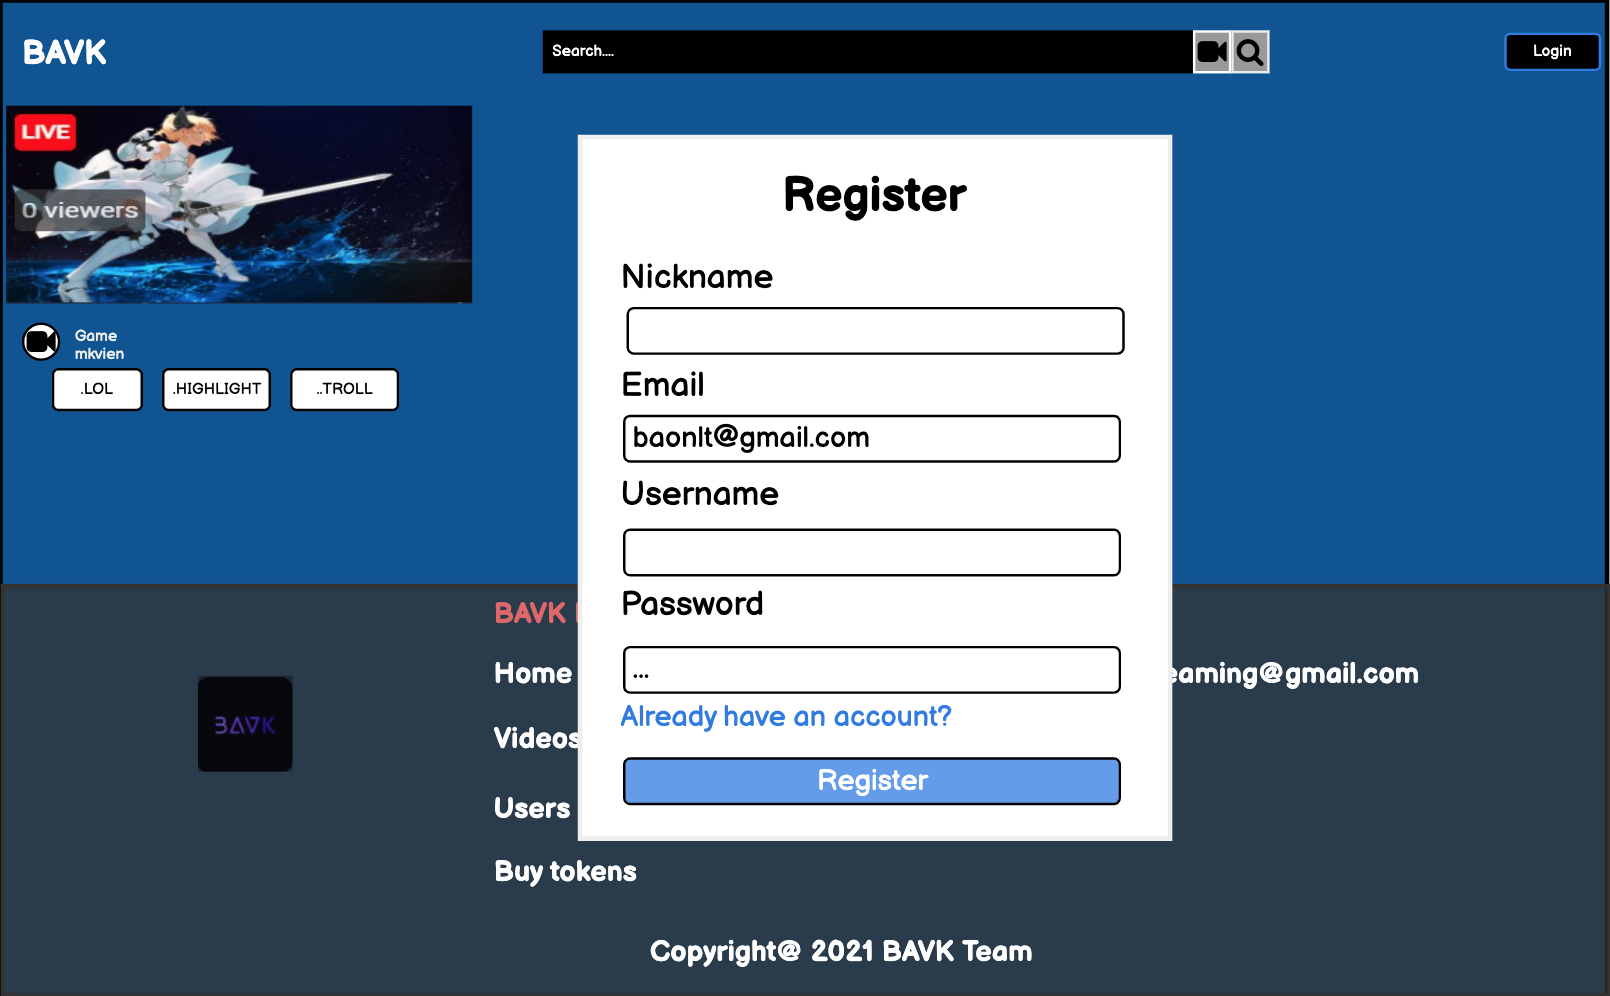
\includegraphics[width=17cm]{{./imgs/register_page}}
		\caption{Trang đăng ký}
	\end{figure}
	\end{center}
	
\begin{center}
\begin{longtabu} to \textwidth {| m{1cm} | m{4cm} | m{3cm} | m{7cm} |}
\caption{Mô tả dialog Đăng nhập/Đăng ký/Đổi mật khẩu} \\
    \hline \textbf{STT}  & \textbf{Điều khiển} & \textbf{Sự kiện} & \textbf{Mô tả} \\ \hline
    \endfirsthead
    \hline \textbf{STT}  & \textbf{Điều khiển} & \textbf{Sự kiện} & \textbf{Mô tả} \\ \hline
    \endhead
      1 & Username & Input & Tên đăng nhập \\
      \hline
      2 & Password & Input & Mật khẩu đăng nhập \\
      \hline
      3 & Email & Input & Địa chỉ email \\
      \hline
      4 & Username & Input & Tên đăng nhập \\
      \hline
\end{longtabu}
\end{center}
	
	
	\begin{center}
	\begin{figure}[H]
		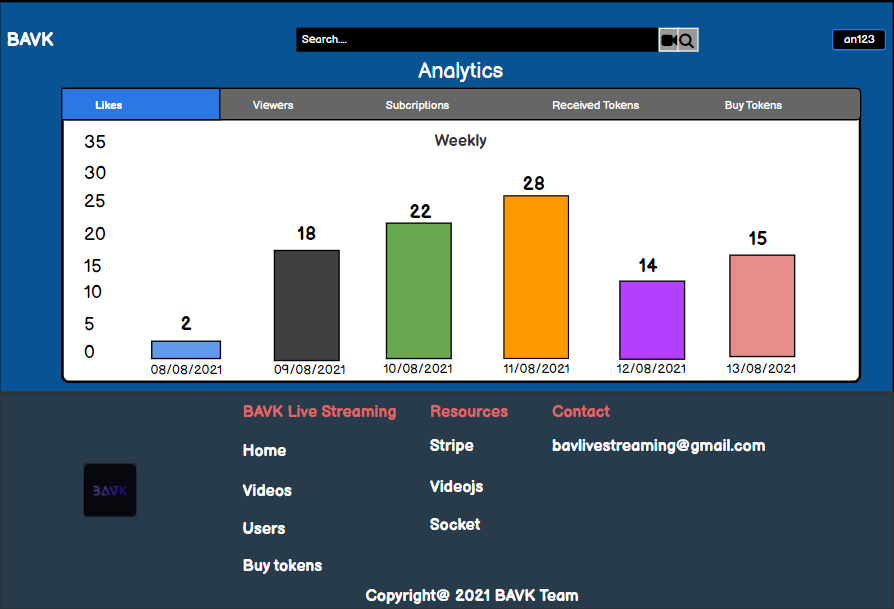
\includegraphics[width=17cm]{{./imgs/analytics}}
		\caption{Trang thống kê}
	\end{figure}
	\end{center}
	
\begin{center}
\begin{longtabu} to \textwidth {| m{1cm} | m{4cm} | m{3cm} | m{7cm} |}
\caption{Mô tả trang danh sách người dùng} \\
    \hline \textbf{STT}  & \textbf{Điều khiển} & \textbf{Sự kiện} & \textbf{Mô tả} \\ \hline
    \endfirsthead
    \hline \textbf{STT}  & \textbf{Điều khiển} & \textbf{Sự kiện} & \textbf{Mô tả} \\ \hline
    \endhead
      1 & Thống kê giao dịch ngân hàng & Initialize & So sánh số lượng tiền nạp vào và tiền rút ra \\
      \hline
      2 & Thống kê donate & Initialize & So sánh số lượng token được donate và donate\\
      \hline
       3 & Thống kê thông tin chung & Initialize/Click & Xem dữ liệu biến động qua các mốc thời gian theo mục được chọn\\
      \hline
\end{longtabu}
\end{center}


	\begin{center}
	\begin{figure}[H]
		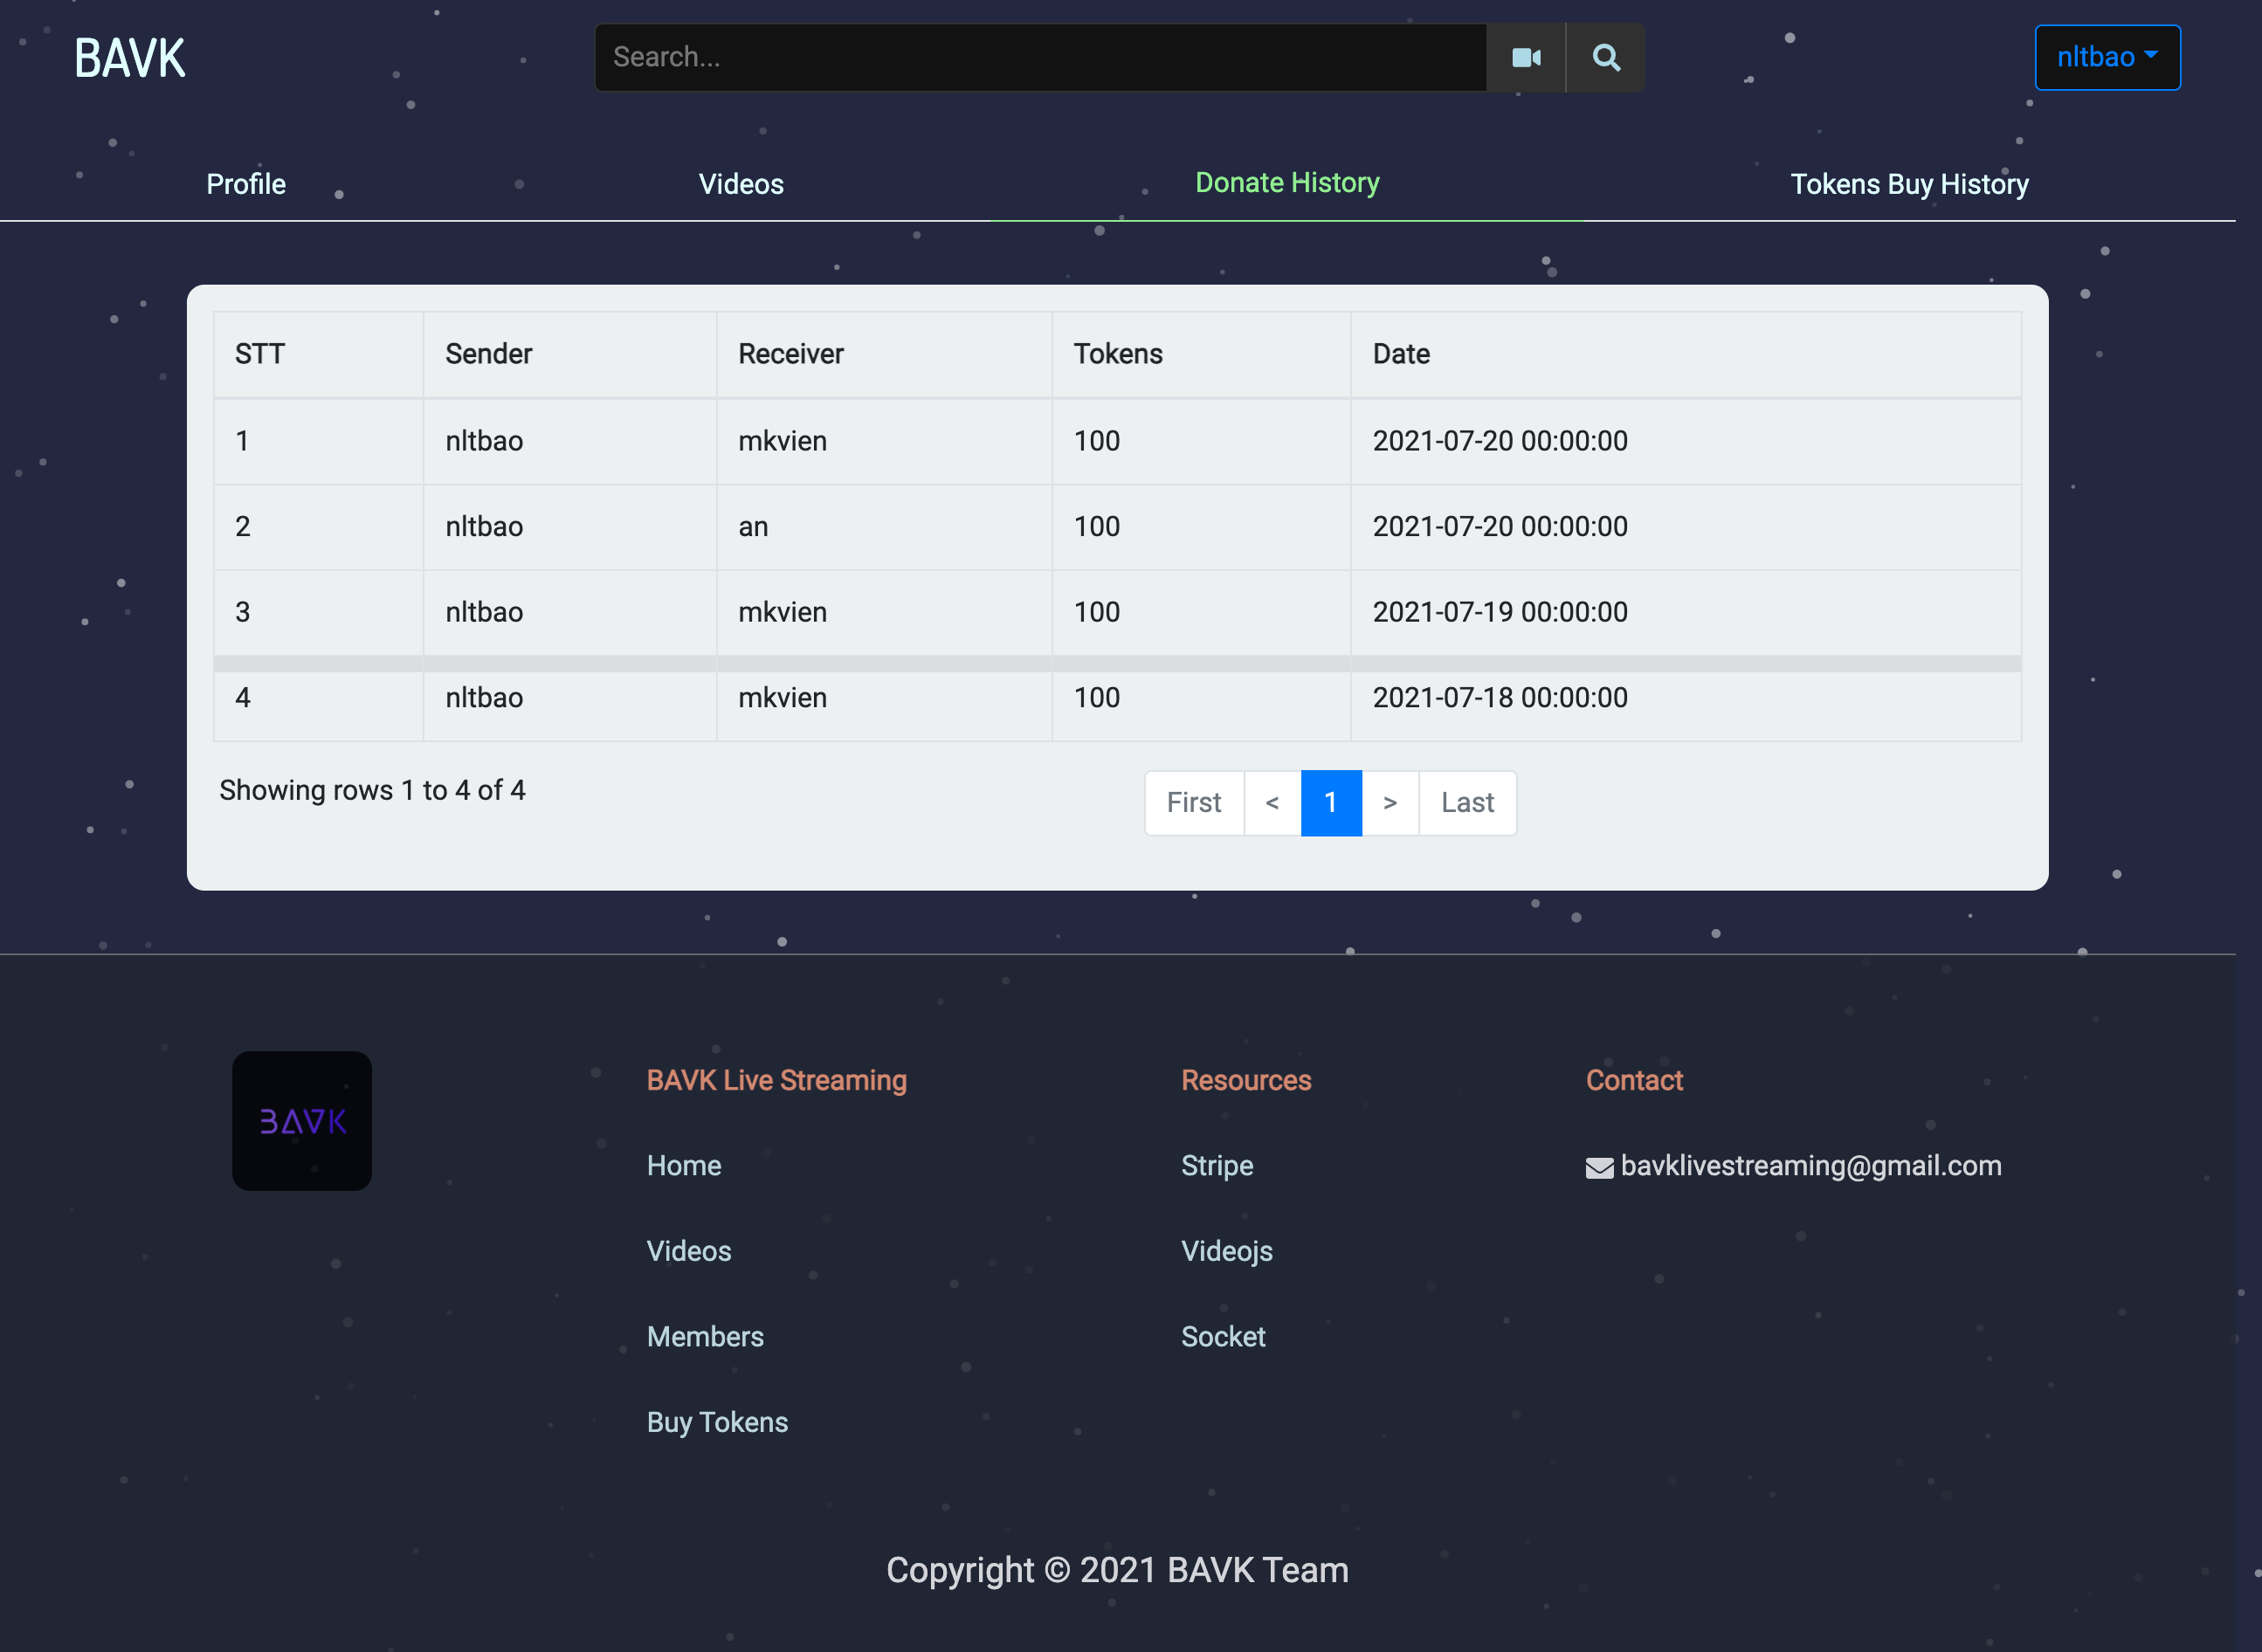
\includegraphics[width=17cm]{{./imgs/history_donate}}
		\caption{Trang lịch sử donate}
	\end{figure}
	\end{center}
	
\begin{center}
\begin{longtabu} to \textwidth {| m{1cm} | m{4cm} | m{3cm} | m{7cm} |}
\caption{Mô tả trang lịch sử donate} \\
    \hline \textbf{STT}  & \textbf{Điều khiển} & \textbf{Sự kiện} & \textbf{Mô tả} \\ \hline
    \endfirsthead
    \hline \textbf{STT}  & \textbf{Điều khiển} & \textbf{Sự kiện} & \textbf{Mô tả} \\ \hline
    \endhead
      1 & Xem lịch sử  & Initialize & Cho phép người dùng xem thông tin lịch sử donate\\
      \hline
\end{longtabu}
\end{center}

	\begin{center}
	\begin{figure}[H]
		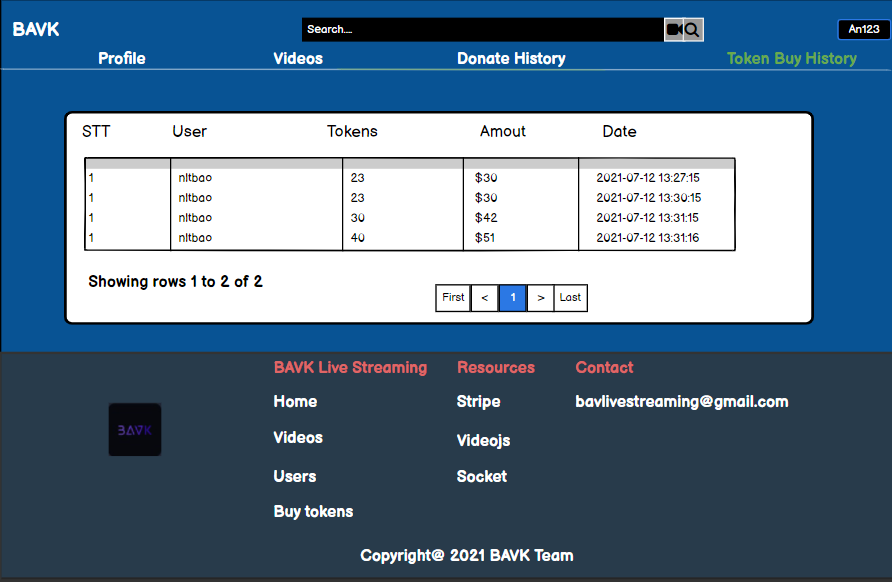
\includegraphics[width=17cm]{{./imgs/history_token}}
		\caption{Trang lịch sử token}
	\end{figure}
	\end{center}

\begin{center}
\begin{longtabu} to \textwidth {| m{1cm} | m{4cm} | m{3cm} | m{7cm} |}
\caption{Mô tả trang lịch sử token} \\
    \hline \textbf{STT}  & \textbf{Điều khiển} & \textbf{Sự kiện} & \textbf{Mô tả} \\ \hline
    \endfirsthead
    \hline \textbf{STT}  & \textbf{Điều khiển} & \textbf{Sự kiện} & \textbf{Mô tả} \\ \hline
    \endhead
      1 & Xem lịch sử  & Initialize & Cho phép người dùng xem thông tin lịch sử mua token\\
      \hline
\end{longtabu}
\end{center}

	\begin{center}
	\begin{figure}[H]
		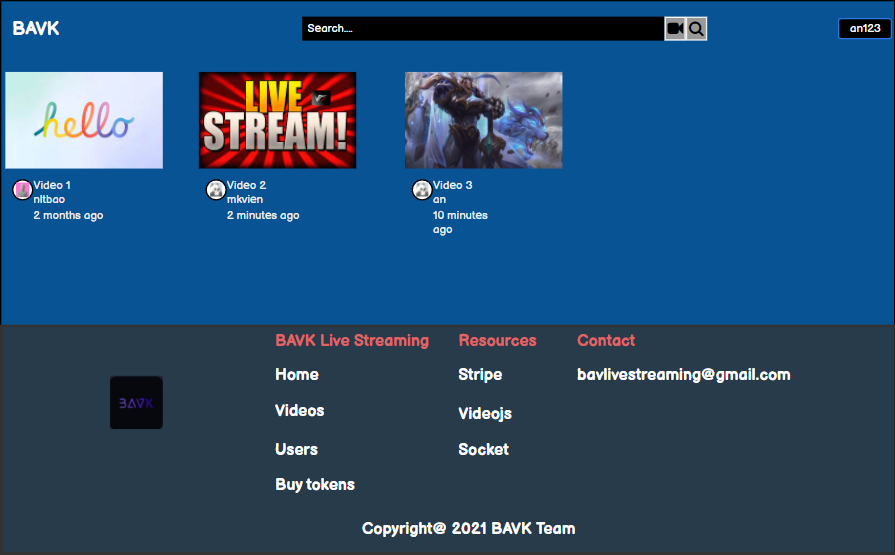
\includegraphics[width=17cm]{{./imgs/page_video.png}}
		\caption{Trang danh sách video}
	\end{figure}
	\end{center}

\begin{center}
\begin{longtabu} to \textwidth {| m{1cm} | m{4cm} | m{3cm} | m{7cm} |}
\caption{Mô tả trang danh sách videos} \\
    \hline \textbf{STT}  & \textbf{Điều khiển} & \textbf{Sự kiện} & \textbf{Mô tả} \\ \hline
    \endfirsthead
    \hline \textbf{STT}  & \textbf{Điều khiển} & \textbf{Sự kiện} & \textbf{Mô tả} \\ \hline
    \endhead
      1 & Danh sách video  & Initialize & Hiển thị các video được tạo ra từ ghi hình của user\\
      \hline
      2 & Thay đổi thông tin video & Click/Input & Cho phép user thay đổi tiêu đề của video \\
      \hline
\end{longtabu}
\end{center}

	\begin{center}
	\begin{figure}[H]
		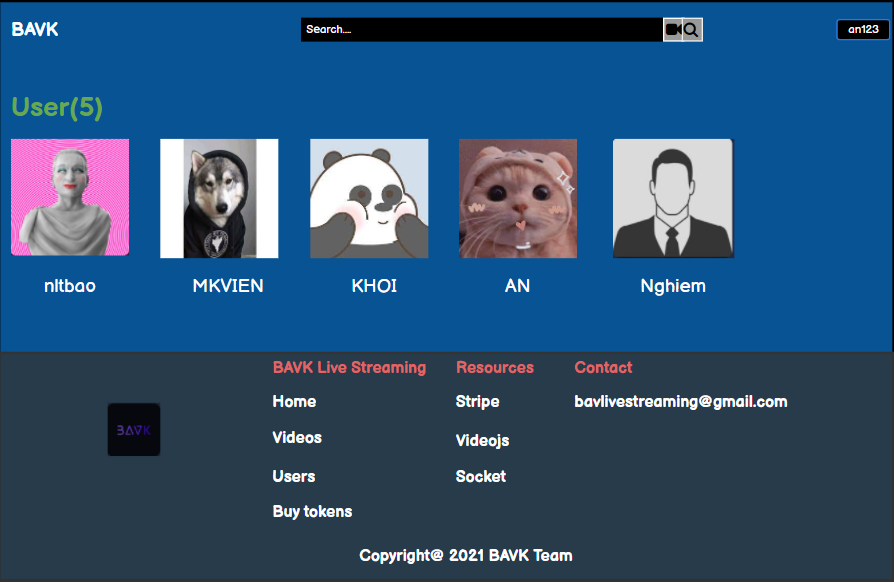
\includegraphics[width=17cm]{{./imgs/page_user}}
		\caption{Trang danh sách người dùng}
	\end{figure}
	\end{center}

\begin{center}
\begin{longtabu} to \textwidth {| m{1cm} | m{4cm} | m{3cm} | m{7cm} |}
\caption{Mô tả trang danh sách người dùng} \\
    \hline \textbf{STT}  & \textbf{Điều khiển} & \textbf{Sự kiện} & \textbf{Mô tả} \\ \hline
    \endfirsthead
    \hline \textbf{STT}  & \textbf{Điều khiển} & \textbf{Sự kiện} & \textbf{Mô tả} \\ \hline
    \endhead
      1 & Danh sách người dùng  & Initialize & Hiển thị toàn bộ danh sách người dùng \\
      \hline
      2 & Xem thông tin hồ sơ người dùng & Click & Điều hướng tới trang hồ sơ của người dùng \\
      \hline
\end{longtabu}
\end{center}


\section{Thiết Kế Dữ Liệu}
\subsection{Sơ đồ thực thể ERD}
\subsubsection{Tổng quan ERD}
	\begin{center}
		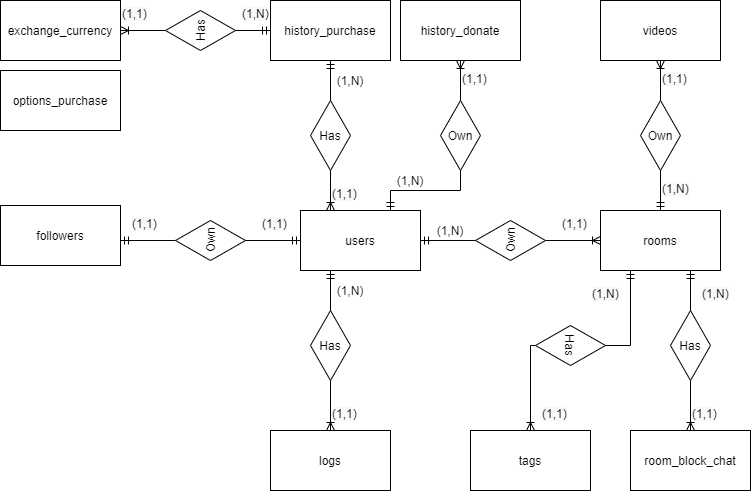
\includegraphics[width=17cm]{{./imgs/erd_overview}}
	\end{center}
	
\subsubsection{Chi tiết ERD}
	\begin{center}
		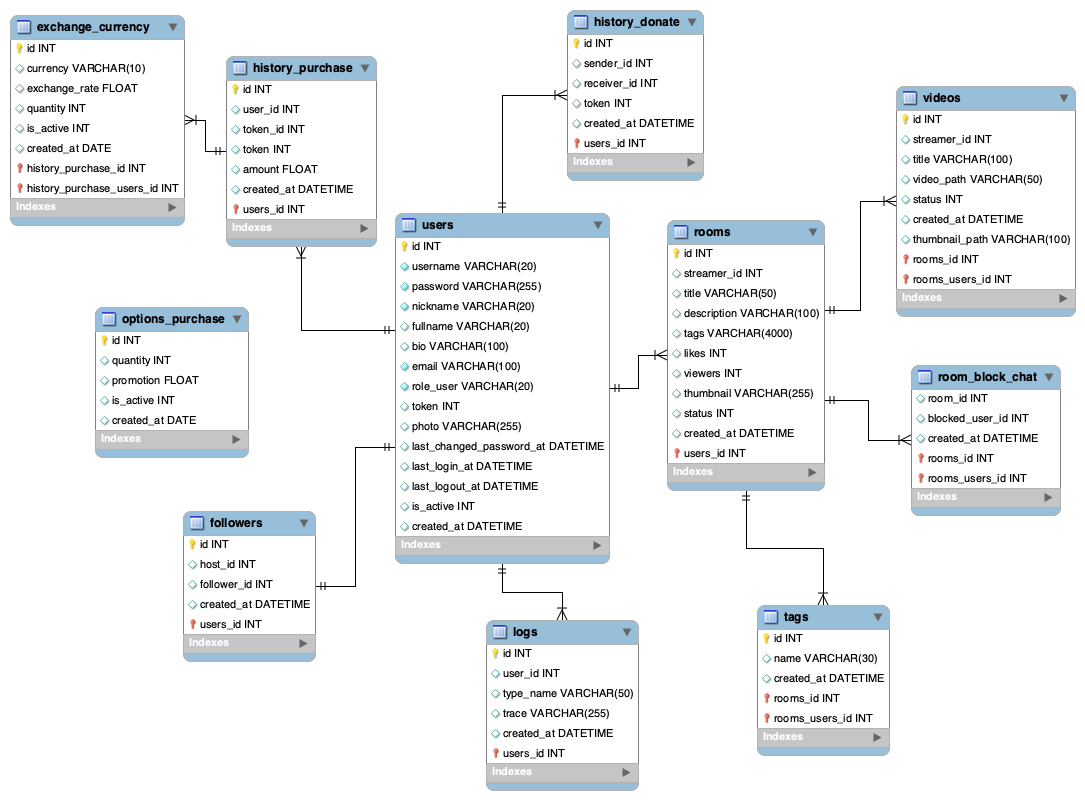
\includegraphics[width=17cm]{{./imgs/erd}}
	\end{center}
	
\subsubsection{Chi tiết các thực thể}


%%%%%%%% USERS %%%%%%%%
\begin{center}
\begin{longtabu} to \textwidth {| m{3cm} | m{3cm} | m{5cm} | m{4cm} |}
\caption{Thực thể Users} \\
   \hline \textbf{Thuộc tính}  & \textbf{Kiểu} & \textbf{Mô tả} & \textbf{Ràng buộc} \\ \hline
   \endfirsthead
   \hline \textbf{Thuộc tính}  & \textbf{Kiểu} & \textbf{Mô tả} & \textbf{Ràng buộc} \\ \hline
   \endhead
      id & int  & Mã loại & PK,Tự tăng
      \\ \hline
      username & varchar(20) & Tên đăng nhập & NOT NULL 
      \\ \hline
      password & varchar(255) & Mật khẩu đăng nhập & NOT NULL
      \\ \hline
      nickname & nvarchar(20) & Biệt danh & NOT NULL
      \\ \hline
      fullname & nvarchar(20) & Họ và tên & NULL
      \\ \hline
      role\_user & varchar(20) & Vai trò người dùng& NOT NULL
      \\ \hline
      token & int & Tổng số \quotes{xèng} & NOT NULL
      \\ \hline
      email & varchar(20) & Email người dùng & NOT NULL
      \\ \hline
      gender & nvarchar(10) & Giới tính & NULL
      \\ \hline
      mobile & varchar(20) & Số điện thoại & NULL
      \\ \hline
      photo & varchar(100) & Ảnh avatar & NULL
      \\ \hline
      address & nvarchar(100) & Địa chỉ & NULL
      \\ \hline
      birthday & date & Ngày sinh & NULL
      \\ \hline
      last\_login\_at & datetime & Thời điểm lần cuối đăng nhập & NULL
      \\ \hline
      last\_logout\_at & datetime & Thời điểm lần cuối đăng xuất & NULL
      \\ \hline
      last\_changed \_password\_at & datetime & Thời điểm lần cuối đổi mật khẩu & NULL
      \\ \hline
      is\_active & int & Trạng thái tài khoản & NOT NULL
      \\ \hline
\end{longtabu}
\end{center}


%%%%%%%% ROOMS %%%%%%%%
\begin{center}
\begin{longtabu} to \textwidth {| m{3cm} | m{3cm} | m{5cm} | m{4cm} |}
\caption{Thực thể Rooms} \\
   \hline \textbf{Thuộc tính}  & \textbf{Kiểu} & \textbf{Mô tả} & \textbf{Ràng buộc} \\ \hline
   \endfirsthead
   \hline \textbf{Thuộc tính}  & \textbf{Kiểu} & \textbf{Mô tả} & \textbf{Ràng buộc} \\ \hline
   \endhead
      id & int  & Mã loại & PK,Tự tăng
      \\ \hline
      streamer\_id & int & Id streamer & NOT NULL 
      \\ \hline
      title & nvarchar(50) & Tiêu đề phòng & NOT NULL
      \\ \hline
      description & nvarchar(100) & Mô tả phòng & NULL
      \\ \hline
      tags & nvarchar(max) & Chủ đề phòng & NULL
      \\ \hline
      likes & int & Số lượt yêu thích & NOT NULL
      \\ \hline
      viewers & int & Số lượt ghé thăm & NOT NULL
      \\ \hline
      thumbnail & varchar(100) & Snapshot của phòng & NOT NULL
      \\ \hline
      status & int & Trạng thái phòng & NOT NULL
      \\ \hline
      created\_at & datetime & Ngày tạo & NOT NULL
      \\ \hline
\end{longtabu}
\end{center}

%%%%%%%% VIDEOS %%%%%%%%
\begin{center}
\begin{longtabu} to \textwidth {| m{3cm} | m{3cm} | m{5cm} | m{4cm} |}
\caption{Thực thể Videos} \\
   \hline \textbf{Thuộc tính}  & \textbf{Kiểu} & \textbf{Mô tả} & \textbf{Ràng buộc} \\ \hline
   \endfirsthead
   \hline \textbf{Thuộc tính}  & \textbf{Kiểu} & \textbf{Mô tả} & \textbf{Ràng buộc} \\ \hline
   \endhead
      id & int  & Mã loại & PK,Tự tăng
      \\ \hline
      streamer\_id & int & Id streamer & NOT NULL 
      \\ \hline
      title & nvarchar(50) & Tiêu đề phòng & NOT NULL
      \\ \hline
      video\_path & varchar(100) & Đường dẫn tới video & NOT NULL
      \\ \hline
      status & int & Trạng thái video & NOT NULL
      \\ \hline
      created\_at & datetime & Ngày tạo & NOT NULL
      \\ \hline
\end{longtabu}
\end{center}

%%%%%%%% ROOM_BLOCK_CHAT %%%%%%%%
\begin{center}
\begin{longtabu} to \textwidth {| m{3cm} | m{3cm} | m{5cm} | m{4cm} |}
\caption{Thực thể Room Block Chat} \\
   \hline \textbf{Thuộc tính}  & \textbf{Kiểu} & \textbf{Mô tả} & \textbf{Ràng buộc} \\ \hline
   \endfirsthead
   \hline \textbf{Thuộc tính}  & \textbf{Kiểu} & \textbf{Mô tả} & \textbf{Ràng buộc} \\ \hline
   \endhead
      room\_id & int & Mã loại  & PK,Tự tăng
      \\ \hline
      blocked\_userId & int & Id user & NOT NULL
      \\ \hline
      created\_at & datetime & Ngày tạo & NOT NULL
      \\ \hline
\end{longtabu}
\end{center}

%%%%%%%% TAGS %%%%%%%%
\begin{center}
\begin{longtabu} to \textwidth {| m{3cm} | m{3cm} | m{5cm} | m{4cm} |}
\caption{Thực thể Tags} \\
   \hline \textbf{Thuộc tính}  & \textbf{Kiểu} & \textbf{Mô tả} & \textbf{Ràng buộc} \\ \hline
   \endfirsthead
   \hline \textbf{Thuộc tính}  & \textbf{Kiểu} & \textbf{Mô tả} & \textbf{Ràng buộc} \\ \hline
   \endhead
      id & int  & Mã loại & PK,Tự tăng
      \\ \hline
      name & nvarchar(20) & Tên chủ đề & NOT NULL 
      \\ \hline
      created\_at & datetime & Ngày tạo & NOT NULL
      \\ \hline
\end{longtabu}
\end{center}

%%%%%%%% HISTORY DONATE %%%%%%%%
\begin{center}
\begin{longtabu} to \textwidth {| m{3cm} | m{3cm} | m{5cm} | m{4cm} |}
\caption{Thực thể History Donate} \\
   \hline \textbf{Thuộc tính}  & \textbf{Kiểu} & \textbf{Mô tả} & \textbf{Ràng buộc} \\ \hline
   \endfirsthead
   \hline \textbf{Thuộc tính}  & \textbf{Kiểu} & \textbf{Mô tả} & \textbf{Ràng buộc} \\ \hline
   \endhead
      id & int  & Mã loại & PK,Tự tăng
      \\ \hline
      sender\_id & int & Id người gửi & NOT NULL 
      \\ \hline
      receiver\_id & int & Id người nhận  & NOT NULL 
      \\ \hline
      token & int & Số lượng \quotes{Xèng} & NOT NULL
      \\ \hline
      created\_at & datetime & Ngày tạo & NOT NULL
      \\ \hline
\end{longtabu}
\end{center}

%%%%%%%% HISTORY PURCHASE %%%%%%%%
\begin{center}
\begin{longtabu} to \textwidth {| m{3cm} | m{3cm} | m{5cm} | m{4cm} |}
\caption{Thực thể History Purchase} \\
   \hline \textbf{Thuộc tính}  & \textbf{Kiểu} & \textbf{Mô tả} & \textbf{Ràng buộc} \\ \hline
   \endfirsthead
   \hline \textbf{Thuộc tính}  & \textbf{Kiểu} & \textbf{Mô tả} & \textbf{Ràng buộc} \\ \hline
   \endhead
      id & int  & Mã loại & PK,Tự tăng
      \\ \hline
      user\_id & int & Id người dùng & NOT NULL 
      \\ \hline
      token\_id & int & Id tỉ giá tiền tệ  & NOT NULL 
      \\ \hline
      amount & float & Số tiền & NOT NULL
       \\ \hline
      token & int & Số lượng \quotes{Xèng} & NOT NULL
      \\ \hline
      created\_at & datetime & Ngày tạo & NOT NULL
      \\ \hline
\end{longtabu}
\end{center}

%%%%%%%% EXCHANGE CURRENCY %%%%%%%%
\begin{center}
\begin{longtabu} to \textwidth {| m{3cm} | m{3cm} | m{5cm} | m{4cm} |}
\caption{Thực thể Exchange Currency} \\
   \hline \textbf{Thuộc tính}  & \textbf{Kiểu} & \textbf{Mô tả} & \textbf{Ràng buộc} \\ \hline
   \endfirsthead
   \hline \textbf{Thuộc tính}  & \textbf{Kiểu} & \textbf{Mô tả} & \textbf{Ràng buộc} \\ \hline
   \endhead
      id & int  & Mã loại & PK,Tự tăng
      \\ \hline
      currency & varchar(10) & Đơn vị tiền tệ (USD,VND,...) & NOT NULL 
      \\ \hline
      exchange\_rate & float & Tỉ giá tiền tệ  & NOT NULL 
      \\ \hline
      quantity & int & Số \quotes{Xèng} dự vào tỉ giá & NOT NULL
       \\ \hline
      is\_active & int & Trạng thái & NOT NULL
      \\ \hline
      created\_at & datetime & Ngày tạo & NOT NULL
      \\ \hline
\end{longtabu}
\end{center}

%%%%%%%% OPTION PURCHASE %%%%%%%%
\begin{center}
\begin{longtabu} to \textwidth {| m{3cm} | m{3cm} | m{5cm} | m{4cm} |}
\caption{Thực thể Option Purchase} \\
   \hline \textbf{Thuộc tính}  & \textbf{Kiểu} & \textbf{Mô tả} & \textbf{Ràng buộc} \\ \hline
   \endfirsthead
   \hline \textbf{Thuộc tính}  & \textbf{Kiểu} & \textbf{Mô tả} & \textbf{Ràng buộc} \\ \hline
   \endhead
      id & int  & Mã loại & PK,Tự tăng
      \\ \hline
      quantity & int & Số \quotes{Xèng} & NOT NULL
      \\ \hline
      promotion & float & Phần trăm khuyến mãi & NOT NULL 
       \\ \hline
      is\_active & int & Trạng thái & NOT NULL
      \\ \hline
      created\_at & datetime & Ngày tạo & NOT NULL
      \\ \hline
\end{longtabu}
\end{center}

%%%%%%%% FOLLOWERS  %%%%%%%%
\begin{center}
\begin{longtabu} to \textwidth {| m{3cm} | m{3cm} | m{5cm} | m{4cm} |}
\caption{Thực thể Followers} \\
   \hline \textbf{Thuộc tính}  & \textbf{Kiểu} & \textbf{Mô tả} & \textbf{Ràng buộc} \\ \hline
   \endfirsthead
   \hline \textbf{Thuộc tính}  & \textbf{Kiểu} & \textbf{Mô tả} & \textbf{Ràng buộc} \\ \hline
   \endhead
      id & int  & Mã loại & PK,Tự tăng
      \\ \hline
      host\_id & int & Id người dùng được theo dõi & NOT NULL
      \\ \hline
      follower\_id & int & Id người dùng theo dõi & NOT NULL 
       \\ \hline
      created\_at & datetime & Ngày tạo & NOT NULL
      \\ \hline
\end{longtabu}
\end{center}

%%%%%%%% LOGS  %%%%%%%%
\begin{center}
\begin{longtabu} to \textwidth {| m{3cm} | m{3cm} | m{5cm} | m{4cm} |}
\caption{Thực thể Logs} \\
   \hline \textbf{Thuộc tính}  & \textbf{Kiểu} & \textbf{Mô tả} & \textbf{Ràng buộc} \\ \hline
   \endfirsthead
   \hline \textbf{Thuộc tính}  & \textbf{Kiểu} & \textbf{Mô tả} & \textbf{Ràng buộc} \\ \hline
   \endhead
      id & int  & Mã loại & PK,Tự tăng
      \\ \hline
      user\_id & int & Id người dùng & NOT NULL
      \\ \hline
      type\_name & varchar(15) & Loại truy vấn & NOT NULL 
      \\ \hline
      trace & nvarchar(max) & Payload truyền tới server & NOT NULL 
       \\ \hline
      created\_at & datetime & Ngày tạo & NOT NULL
      \\ \hline
\end{longtabu}
\end{center}


%%%%%%%%%%%%%%%%%%% Stored Procedure %%%%%%%%%%%%%%%%%%%%%%%%%

\section{Stored Procedure}

\begin{center}
	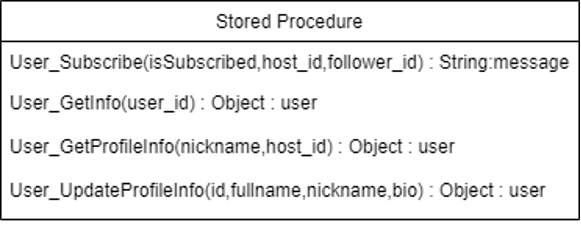
\includegraphics[width=17cm]{{./imgs/diagrams/user_procedure}}
\end{center}

\begin{center}
\begin{longtabu} to \textwidth {| m{3cm} | m{5cm} | m{4cm} | m{4cm} |}
\caption{Các trường} \\
   \hline \textbf{Tên}  & \textbf{Mô tả} & \textbf{Input} & \textbf{Output}  \\ \hline
   \endfirsthead
   \hline \textbf{Tên}  & \textbf{Mô tả} & \textbf{Input} & \textbf{Output}  \\ \hline
   \endhead
      Subscribe & Đăng ký kênh  & isSubscribed: 1 – 0, hostId: địa chỉ kênh, followerId: Id của user & Trạng thái đăng ký
      \\ \hline
      GetInfo & Lấy thông tin tài khoản  & UserId: mã Id của user & Thông tin tài khoản đăng nhập
      \\ \hline
      GetProfileInfo & Lấy thông tin user khác  & Nickname: tên nickname, HostId: địa chỉ host & Thông tin hồ sơ
      \\ \hline
      UpdateProfileInfo & Cập nhật thông tin cá nhân của tài khoản  & Id: mã id tài khoản, Fullname: tên đầy đủ, Nickname: tên nickname, Bio: thông tin thêm & Trạng thái cập nhật
      \\ \hline
\end{longtabu}
\end{center}

\begin{center}
	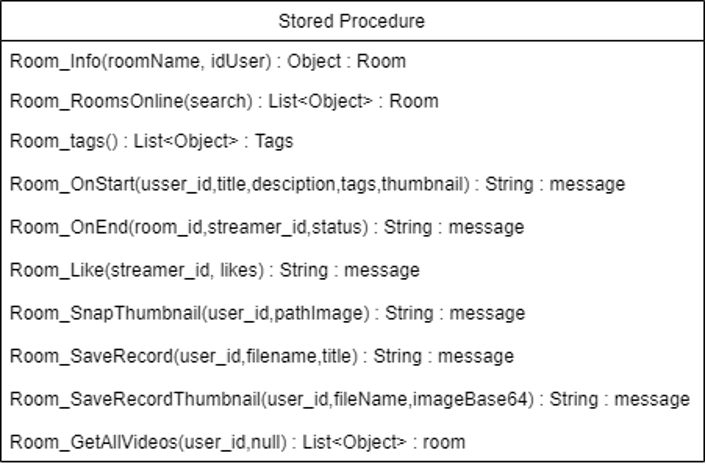
\includegraphics[width=17cm]{{./imgs/diagrams/stream_procedure}}
\end{center}

\begin{center}
\begin{longtabu} to \textwidth {| m{3cm} | m{5cm} | m{4cm} | m{4cm} |}
\caption{Các trường} \\
   \hline \textbf{Tên}  & \textbf{Mô tả} & \textbf{Input} & \textbf{Output}  \\ \hline
   \endfirsthead
   \hline \textbf{Tên}  & \textbf{Mô tả} & \textbf{Input} & \textbf{Output}  \\ \hline
   \endhead
      Info & Lấy thông tin Room  & roomName: tên room, idUser: mã user id & Thông tin phòng
      \\ \hline
      RoomOnline & Tìm kiếm Room  & Search: tên room cần tìm & Danh sách phòng đang online
      \\ \hline
      Tags & Lấy danh sách các tags &  & Danh sách tags
      \\ \hline
      OnStart & Tạo phòng và bắt đầu tạo video  & UserId: mã id của user, Title: chủ đề video, Description: mô tả về video, Tags: tên tags, Thumbnail: ảnh đại diên
 & Thông tin live stream
      \\ \hline
      OnEnd & Kết thúc video & RoomId: mã phòng, StreamerId: mã tài khoản, Status: tình trạng & Thông tin dừng live stream
      \\ \hline
      Like & Thực hiện like video & StreamerId: mã tài khoản, Likes: 1 - 0 & Trạng thái
      \\ \hline
      SnapThumbnail & Snap hình ảnh& UserId: mã tài khoản, pathImage: ảnh & Trạng thái
      \\ \hline
      SaveRecord & Lưu video & UserId: mã tài khoản, fileName: đường dẫn video, title: tên chủ đề & Trạng thái
      \\ \hline
      SaveRecord Thumbnail & Lưu ảnh video & UserId: mã tài khoản, fileName: file video, imageBase64: ảnh & Trạng thái
      \\ \hline
      GetAllVideos & Lấy thông tin tất cả video & UserId: mã tài khoản & Danh sách video
      \\ \hline
\end{longtabu}
\end{center}


\begin{center}
	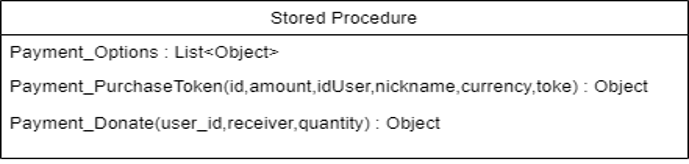
\includegraphics[width=17cm]{{./imgs/diagrams/payment_procedure}}
\end{center}

\begin{center}
\begin{longtabu} to \textwidth {| m{3cm} | m{5cm} | m{4cm} | m{4cm} |}
\caption{Các trường} \\
   \hline \textbf{Tên}  & \textbf{Mô tả} & \textbf{Input} & \textbf{Output}  \\ \hline
   \endfirsthead
   \hline \textbf{Tên}  & \textbf{Mô tả} & \textbf{Input} & \textbf{Output}  \\ \hline
   \endhead
      Option & Danh sách tiền tệ  &  & Danh sách lựa chọn token
      \\ \hline
      PurchaseToken & Mua token & Id: mã tài khoản, Amount: số tiền, idUser: mã id user, nickname: tên nickname, currency: tỉ lệ đổi, toke: số lượng token
 & Thông tin mua token
      \\ \hline
      Donate & Donate token & Userid: mã id user, Receiver: người nhận, Quantity: số lượng
 & Thông tin donate 
      \\ \hline
\end{longtabu}
\end{center}


\begin{center}
	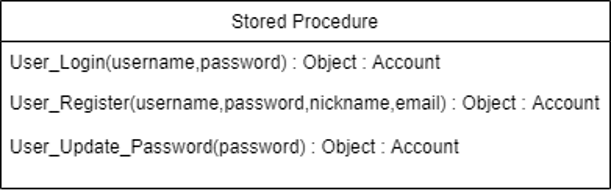
\includegraphics[width=17cm]{{./imgs/diagrams/credential_procedure}}
\end{center}

\begin{center}
\begin{longtabu} to \textwidth {| m{3cm} | m{5cm} | m{4cm} | m{4cm} |}
\caption{Các trường} \\
   \hline \textbf{Tên}  & \textbf{Mô tả} & \textbf{Input} & \textbf{Output}  \\ \hline
   \endfirsthead
   \hline \textbf{Tên}  & \textbf{Mô tả} & \textbf{Input} & \textbf{Output}  \\ \hline
   \endhead
      Login & Đăng nhập tài khoản  & Username: tên đăng nhập, Password: mật khẩu
 & Trạng thái đăng nhập
      \\ \hline
      Register & Đăng ký tài khoản  & Username: tên đăng nhập, Password: mật khẩu, Nickname: tên nickname, Emai: địa chỉ email & Thông tin đăng ký
      \\ \hline
      UpdatePassword & Đổi mật khẩu & Password: mật khẩu & Trạng thái cập nhật
      \\ \hline
\end{longtabu}
\end{center}














